% Options for packages loaded elsewhere
\PassOptionsToPackage{unicode}{hyperref}
\PassOptionsToPackage{hyphens}{url}
%
\documentclass[
  12pt,
]{article}
\usepackage{amsmath,amssymb}
\usepackage{lmodern}
\usepackage{iftex}
\ifPDFTeX
  \usepackage[T1]{fontenc}
  \usepackage[utf8]{inputenc}
  \usepackage{textcomp} % provide euro and other symbols
\else % if luatex or xetex
  \usepackage{unicode-math}
  \defaultfontfeatures{Scale=MatchLowercase}
  \defaultfontfeatures[\rmfamily]{Ligatures=TeX,Scale=1}
\fi
% Use upquote if available, for straight quotes in verbatim environments
\IfFileExists{upquote.sty}{\usepackage{upquote}}{}
\IfFileExists{microtype.sty}{% use microtype if available
  \usepackage[]{microtype}
  \UseMicrotypeSet[protrusion]{basicmath} % disable protrusion for tt fonts
}{}
\makeatletter
\@ifundefined{KOMAClassName}{% if non-KOMA class
  \IfFileExists{parskip.sty}{%
    \usepackage{parskip}
  }{% else
    \setlength{\parindent}{0pt}
    \setlength{\parskip}{6pt plus 2pt minus 1pt}}
}{% if KOMA class
  \KOMAoptions{parskip=half}}
\makeatother
\usepackage{xcolor}
\IfFileExists{xurl.sty}{\usepackage{xurl}}{} % add URL line breaks if available
\IfFileExists{bookmark.sty}{\usepackage{bookmark}}{\usepackage{hyperref}}
\hypersetup{
  pdftitle={Factors affecting inferences on natural mortality and associated environmental effects},
  pdfauthor={Timothy J. Miller1; Andrew Applegate; Greg Britten; Elizabeth N. Brooks; Gavin Fay; Alex Hansell; Christopher M. Legault; Brandon Muffley; Brian C. Stock; John Wiedenmann},
  hidelinks,
  pdfcreator={LaTeX via pandoc}}
\urlstyle{same} % disable monospaced font for URLs
\usepackage[margin=1in]{geometry}
\usepackage{graphicx}
\makeatletter
\def\maxwidth{\ifdim\Gin@nat@width>\linewidth\linewidth\else\Gin@nat@width\fi}
\def\maxheight{\ifdim\Gin@nat@height>\textheight\textheight\else\Gin@nat@height\fi}
\makeatother
% Scale images if necessary, so that they will not overflow the page
% margins by default, and it is still possible to overwrite the defaults
% using explicit options in \includegraphics[width, height, ...]{}
\setkeys{Gin}{width=\maxwidth,height=\maxheight,keepaspectratio}
% Set default figure placement to htbp
\makeatletter
\def\fps@figure{htbp}
\makeatother
\setlength{\emergencystretch}{3em} % prevent overfull lines
\providecommand{\tightlist}{%
  \setlength{\itemsep}{0pt}\setlength{\parskip}{0pt}}
\setcounter{secnumdepth}{5}
\newlength{\cslhangindent}
\setlength{\cslhangindent}{1.5em}
\newlength{\csllabelwidth}
\setlength{\csllabelwidth}{3em}
\newlength{\cslentryspacingunit} % times entry-spacing
\setlength{\cslentryspacingunit}{\parskip}
\newenvironment{CSLReferences}[2] % #1 hanging-ident, #2 entry spacing
 {% don't indent paragraphs
  \setlength{\parindent}{0pt}
  % turn on hanging indent if param 1 is 1
  \ifodd #1
  \let\oldpar\par
  \def\par{\hangindent=\cslhangindent\oldpar}
  \fi
  % set entry spacing
  \setlength{\parskip}{#2\cslentryspacingunit}
 }%
 {}
\usepackage{calc}
\newcommand{\CSLBlock}[1]{#1\hfill\break}
\newcommand{\CSLLeftMargin}[1]{\parbox[t]{\csllabelwidth}{#1}}
\newcommand{\CSLRightInline}[1]{\parbox[t]{\linewidth - \csllabelwidth}{#1}\break}
\newcommand{\CSLIndent}[1]{\hspace{\cslhangindent}#1}
\usepackage{url}
\usepackage{setspace}
%\singlespacing
%\onehalfspacing
\doublespacing
\usepackage{lineno}
\linenumbers
\usepackage[belowskip=0pt,aboveskip=0pt]{caption}
\usepackage{relsize}
\newcommand{\Fmsy}{\ensuremath{F_{\text{MSY}}}\xspace}
\newcommand{\Fspr}[1]{\ensuremath{F_{\text{{#1}\%}}}\xspace}
\newcommand{\afrb}{Alaska Fishery Research Bulletin\xspace}
\newcommand{\ajms}{African Journal of Marine Science\xspace}
\newcommand{\amb}{Advances in Marine Biology\xspace}
\newcommand{\bms}{Bulletin of Marine Science\xspace}
\newcommand{\bjssf}{Bulletin of the Japanese Society of Scientific Fisheries\xspace}
\newcommand{\cb}{Conservation Biology\xspace}
\newcommand{\cjfas}{Canadian Journal of Fisheries and Aquatic Sciences\xspace}
\newcommand{\ea}{Ecological Applications\xspace}
\newcommand{\eer}{Evolutionary Ecology Research\xspace}
\newcommand{\elet}{Ecology Letters\xspace}
\newcommand{\emod}{Ecological Modelling\xspace}
\newcommand{\ebf}{Environmental Biology of Fishes\xspace}
\newcommand{\ff}{Fish and Fisheries\xspace}
\newcommand{\fo}{Fisheries Oceanography\xspace}
\newcommand{\fr}{Fisheries Research\xspace}
\newcommand{\fb}{Fishery Bulletin\xspace}
\newcommand{\ijms}{ICES Journal of Marine Science\xspace}
\newcommand{\iccat}{Collective Volume of Scientific Papers ICCAT\xspace}
\newcommand{\jae}{Journal of Animal Ecology\xspace}
\newcommand{\jai}{Journal of Applied Ichthyology\xspace}
\newcommand{\jdc}{Journal Du Conseil International Pour L'exploration De La Mer\xspace}
\newcommand{\jdcp}{Journal Du Conseil Permanent International Pour L'exploration De La Mer\xspace}
\newcommand{\jembe}{Journal of Experimental Marine Biology and Ecology\xspace}
\newcommand{\jfb}{Journal of Fish Biology\xspace}
\newcommand{\jsr}{Journal of Sea Research\xspace}
\newcommand{\jtb}{Journal of Theoretical Biology\xspace}
\newcommand{\jfrbc}{Journal of the Fisheries Research Board of Canada\xspace}
\newcommand{\jnwafs}{Journal of Northwest Atlantic Fisheries Science\xspace}
\newcommand{\mcf}{Marine and Coastal Fisheries: Dynamics, Management, and Ecosystem Science\xspace}
\newcommand{\mb}{Marine Biology\xspace}
\newcommand{\meps}{Marine Ecology Progress Series\xspace}
\newcommand{\mfr}{Marine Fisheries Review\xspace}
\newcommand{\mpb}{Marine Pollution Bulletin\xspace}
\newcommand{\najfm}{North American Journal of Fisheries Management\xspace}
\newcommand{\nzjmfr}{New Zealand Journal of Marine and Freshwater Research\xspace}
\newcommand{\pnas}{Proceedings of the National Academy of Sciences USA\xspace}
\newcommand{\rpvrciemm}{Rapports et Proc\`es-Verbaux des R\'eunions. Conseil Internationale pour l'Exploration de la Mer\xspace}
\newcommand{\rpvrcpiemm}{Rapports et Proc\`es-Verbaux des R\'eunions. Conseil Permanent Internationale pour l'Exploration de la Mer\xspace}
\newcommand{\rfbf}{Reviews in Fish Biology and Fisheries\xspace}
\newcommand{\sajms}{South African Journal of Marine Science\xspace}
\newcommand{\tafs}{Transactions of the American Fisheries Society\xspace}

\newcommand{\anzjs}{Australian \& New Zealand Journal of Statistics\xspace}
\newcommand{\as}{Applied Statistics\xspace}
\newcommand{\csda}{Computational Statistics \& Data Analysis\xspace}
\newcommand{\ees}{Environmental and Ecological Statistics\xspace}
\newcommand{\jas}{Journal of Applied Statistics\xspace}
\newcommand{\jabes}{Journal of Agricultural, Biological, and Environmental Statistics\xspace}
\newcommand{\jasa}{Journal of the American Statistical Association\xspace}
\newcommand{\jrssb}{Journal of the Royal Statistical Society. Series B\xspace}
\newcommand{\sm}{Statistics in Medicine}

\usepackage{xspace}
\usepackage{bm}
\usepackage{caption,graphics}
\usepackage{graphicx}
\usepackage{makecell}
\renewcommand\figurename{Fig.}
\captionsetup{labelsep=period, singlelinecheck=false}
\newcommand{\changesize}[1]{\fontsize{#1pt}{#1pt}\selectfont}
\renewcommand{\arraystretch}{1.5}
\renewcommand\theadfont{}
\usepackage{booktabs}
\usepackage{longtable}
\usepackage{array}
\usepackage{multirow}
\usepackage{wrapfig}
\usepackage{float}
\usepackage{colortbl}
\usepackage{pdflscape}
\usepackage{tabu}
\usepackage{threeparttable}
\usepackage{threeparttablex}
\usepackage[normalem]{ulem}
\usepackage{makecell}
\usepackage{xcolor}
\ifLuaTeX
  \usepackage{selnolig}  % disable illegal ligatures
\fi
\usepackage[]{natbib}
\bibliographystyle{cjfas2.bst}

\title{Factors affecting inferences on natural mortality and associated
environmental effects}
\author{Timothy J. Miller\textsuperscript{1} \and Andrew
Applegate \and Greg Britten \and Elizabeth N. Brooks \and Gavin
Fay \and Alex Hansell \and Christopher M. Legault \and Brandon
Muffley \and Brian C. Stock \and John Wiedenmann}
\date{}

\begin{document}
\maketitle

\(^1\)corresponding author:
\href{mailto:timothy.j.miller@noaa.gov}{\nolinkurl{timothy.j.miller@noaa.gov}},
Northeast Fisheries Science Center, Woods Hole Laboratory, 166 Water
Street, Woods Hole, MA 02543 USA\\

\pagebreak

\hypertarget{abstract}{%
\subsection*{Abstract}\label{abstract}}
\addcontentsline{toc}{subsection}{Abstract}

\hypertarget{keywords}{%
\subsubsection*{Keywords}\label{keywords}}
\addcontentsline{toc}{subsubsection}{Keywords}

\pagebreak

\hypertarget{introduction}{%
\section*{Introduction}\label{introduction}}
\addcontentsline{toc}{section}{Introduction}

Here we conduct a simulation study with operating models varying by
degree of observation error uncertainty, sources of process error (M or
survival), fishing history, temporal variation in environmental
covariates, and magnitude of the effect of the covariate on natural
mortality. The simulations from these operating models are fitted with
estimating models that make alternative assumptions for sources of
process error (M, NAA), and whether (mean) M is estimated. We evaluate
whether AIC can correctly determine the correct source of process error
and stock effects on recruitment. We also evaluate the degree of bias in
the outputs of the assessment model that are important for management.

\hypertarget{methods}{%
\section*{Methods}\label{methods}}
\addcontentsline{toc}{section}{Methods}

We used the WHAM package
\citep[][commit 77bbd94]{millerstock20,stockmiller21} to configure all
operating models and estimation models. This packages has also been used
to configure operating and estimating models for closed loop simulations
evaluating index-based assessment methods \citep{legaultetal23} and is
used for management of haddock, butterfish, plaice, bluefish in the
Northeast US.

We completed a simulation study with a number of operating models. Many
of the characteristics of the operating models are the same as those
used by \citet{milleretal_wp}.

288 total operating models. We simulated 100 data sets for each
operating model. For each simulated data set we fit a set of 12
estimating models.

\hypertarget{operating-models}{%
\subsection*{Operating models}\label{operating-models}}
\addcontentsline{toc}{subsection}{Operating models}

\hypertarget{population}{%
\subsubsection*{Population}\label{population}}
\addcontentsline{toc}{subsubsection}{Population}

The population model tracks 10 age classes: ages 1 to 10+ and we assume
spawning occurs 1/4 of the way through the year. The maturity at age was
a logistic curve with a50 = 2.89 and slope = 0.88 and assumed known in
all estimation models (Figure \ref{om_maturity}).

\begin{figure}
\caption{The proportion mature at age assumed for the population in all operating and estimating models.}\label{om_maturity}
\begin{center}
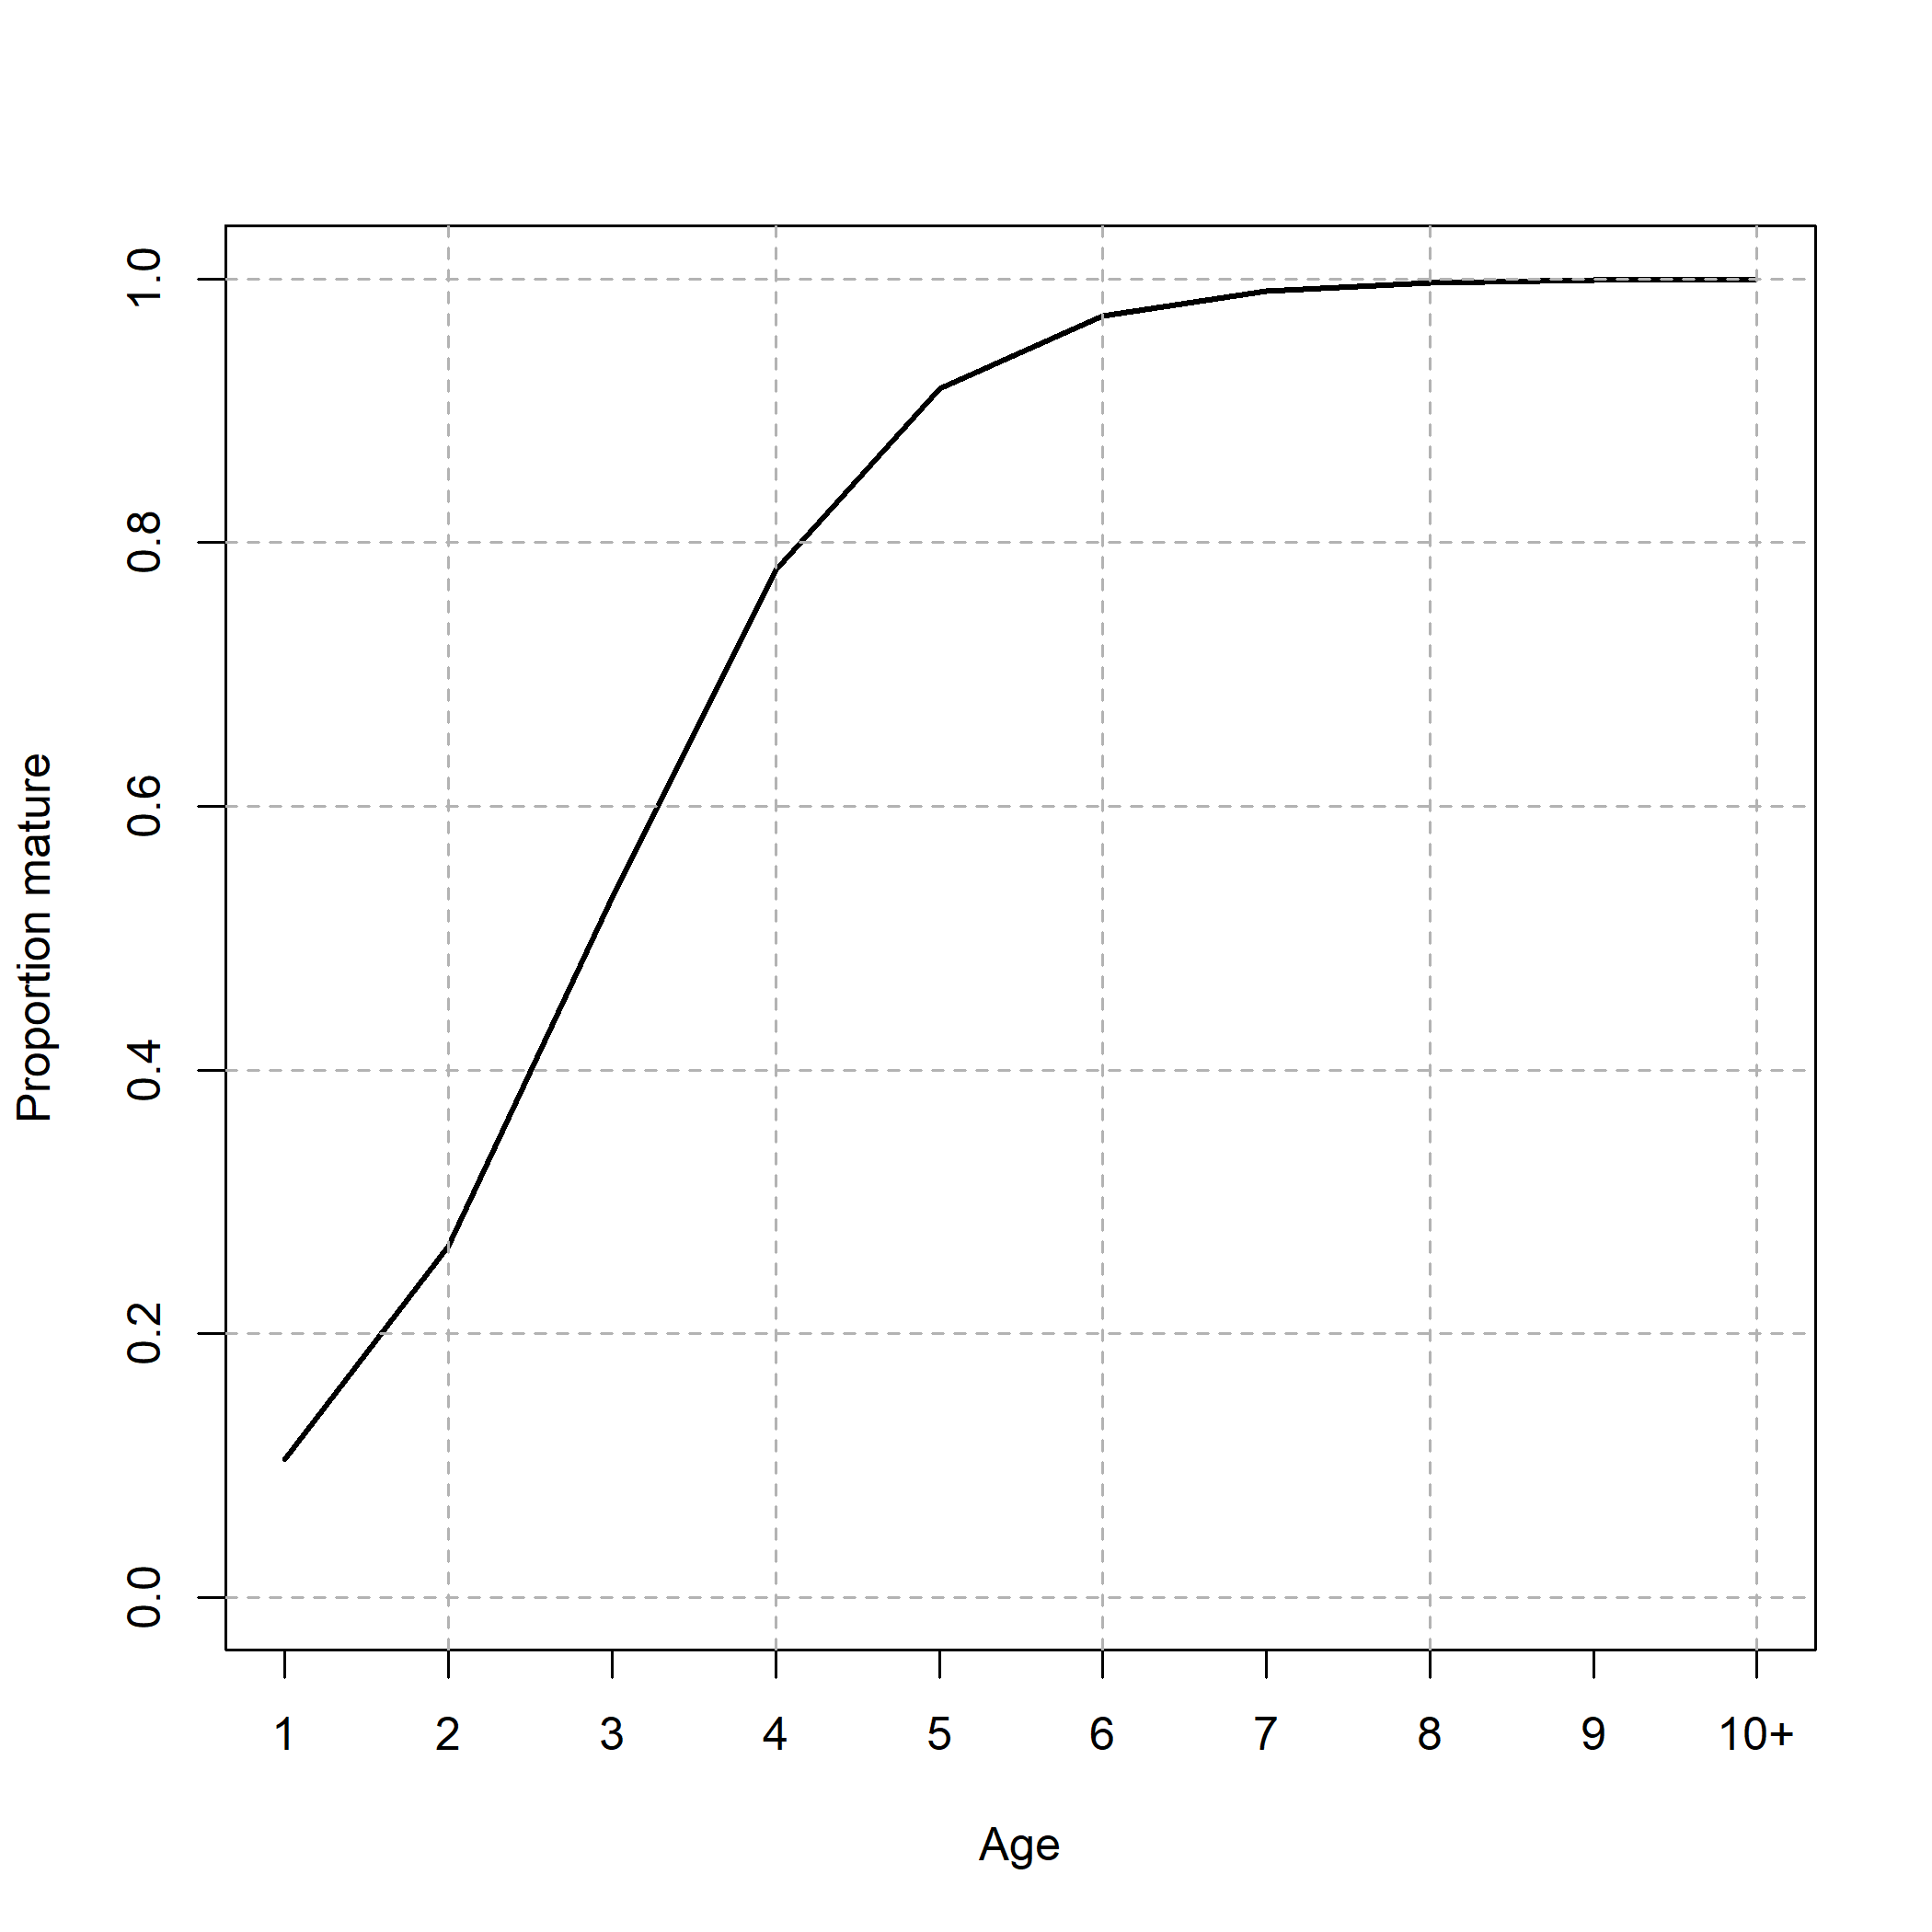
\includegraphics[width = \textwidth]{om_maturity.png}
\end{center}
\end{figure}

Weight at age was generated with a LVB growth function \[
L_a = L_{\infty}\left(1 - e^{-k(a - t_0)}\right)
\] where \(t_0 = 0\), \(L_\infty = 85\), and \(k = 0.3\), and a L-W
relationship such that \[
W_a = \theta_1 L_a^{\theta_2}
\] where \(\theta_1 = e^{-12.1}\) and \(\theta_2 = 3.2\) (Figure
\ref{om_waa}).

\begin{figure}
\caption{The weight at age assumed for the population in all operating and estimating models.}\label{om_waa}
\begin{center}
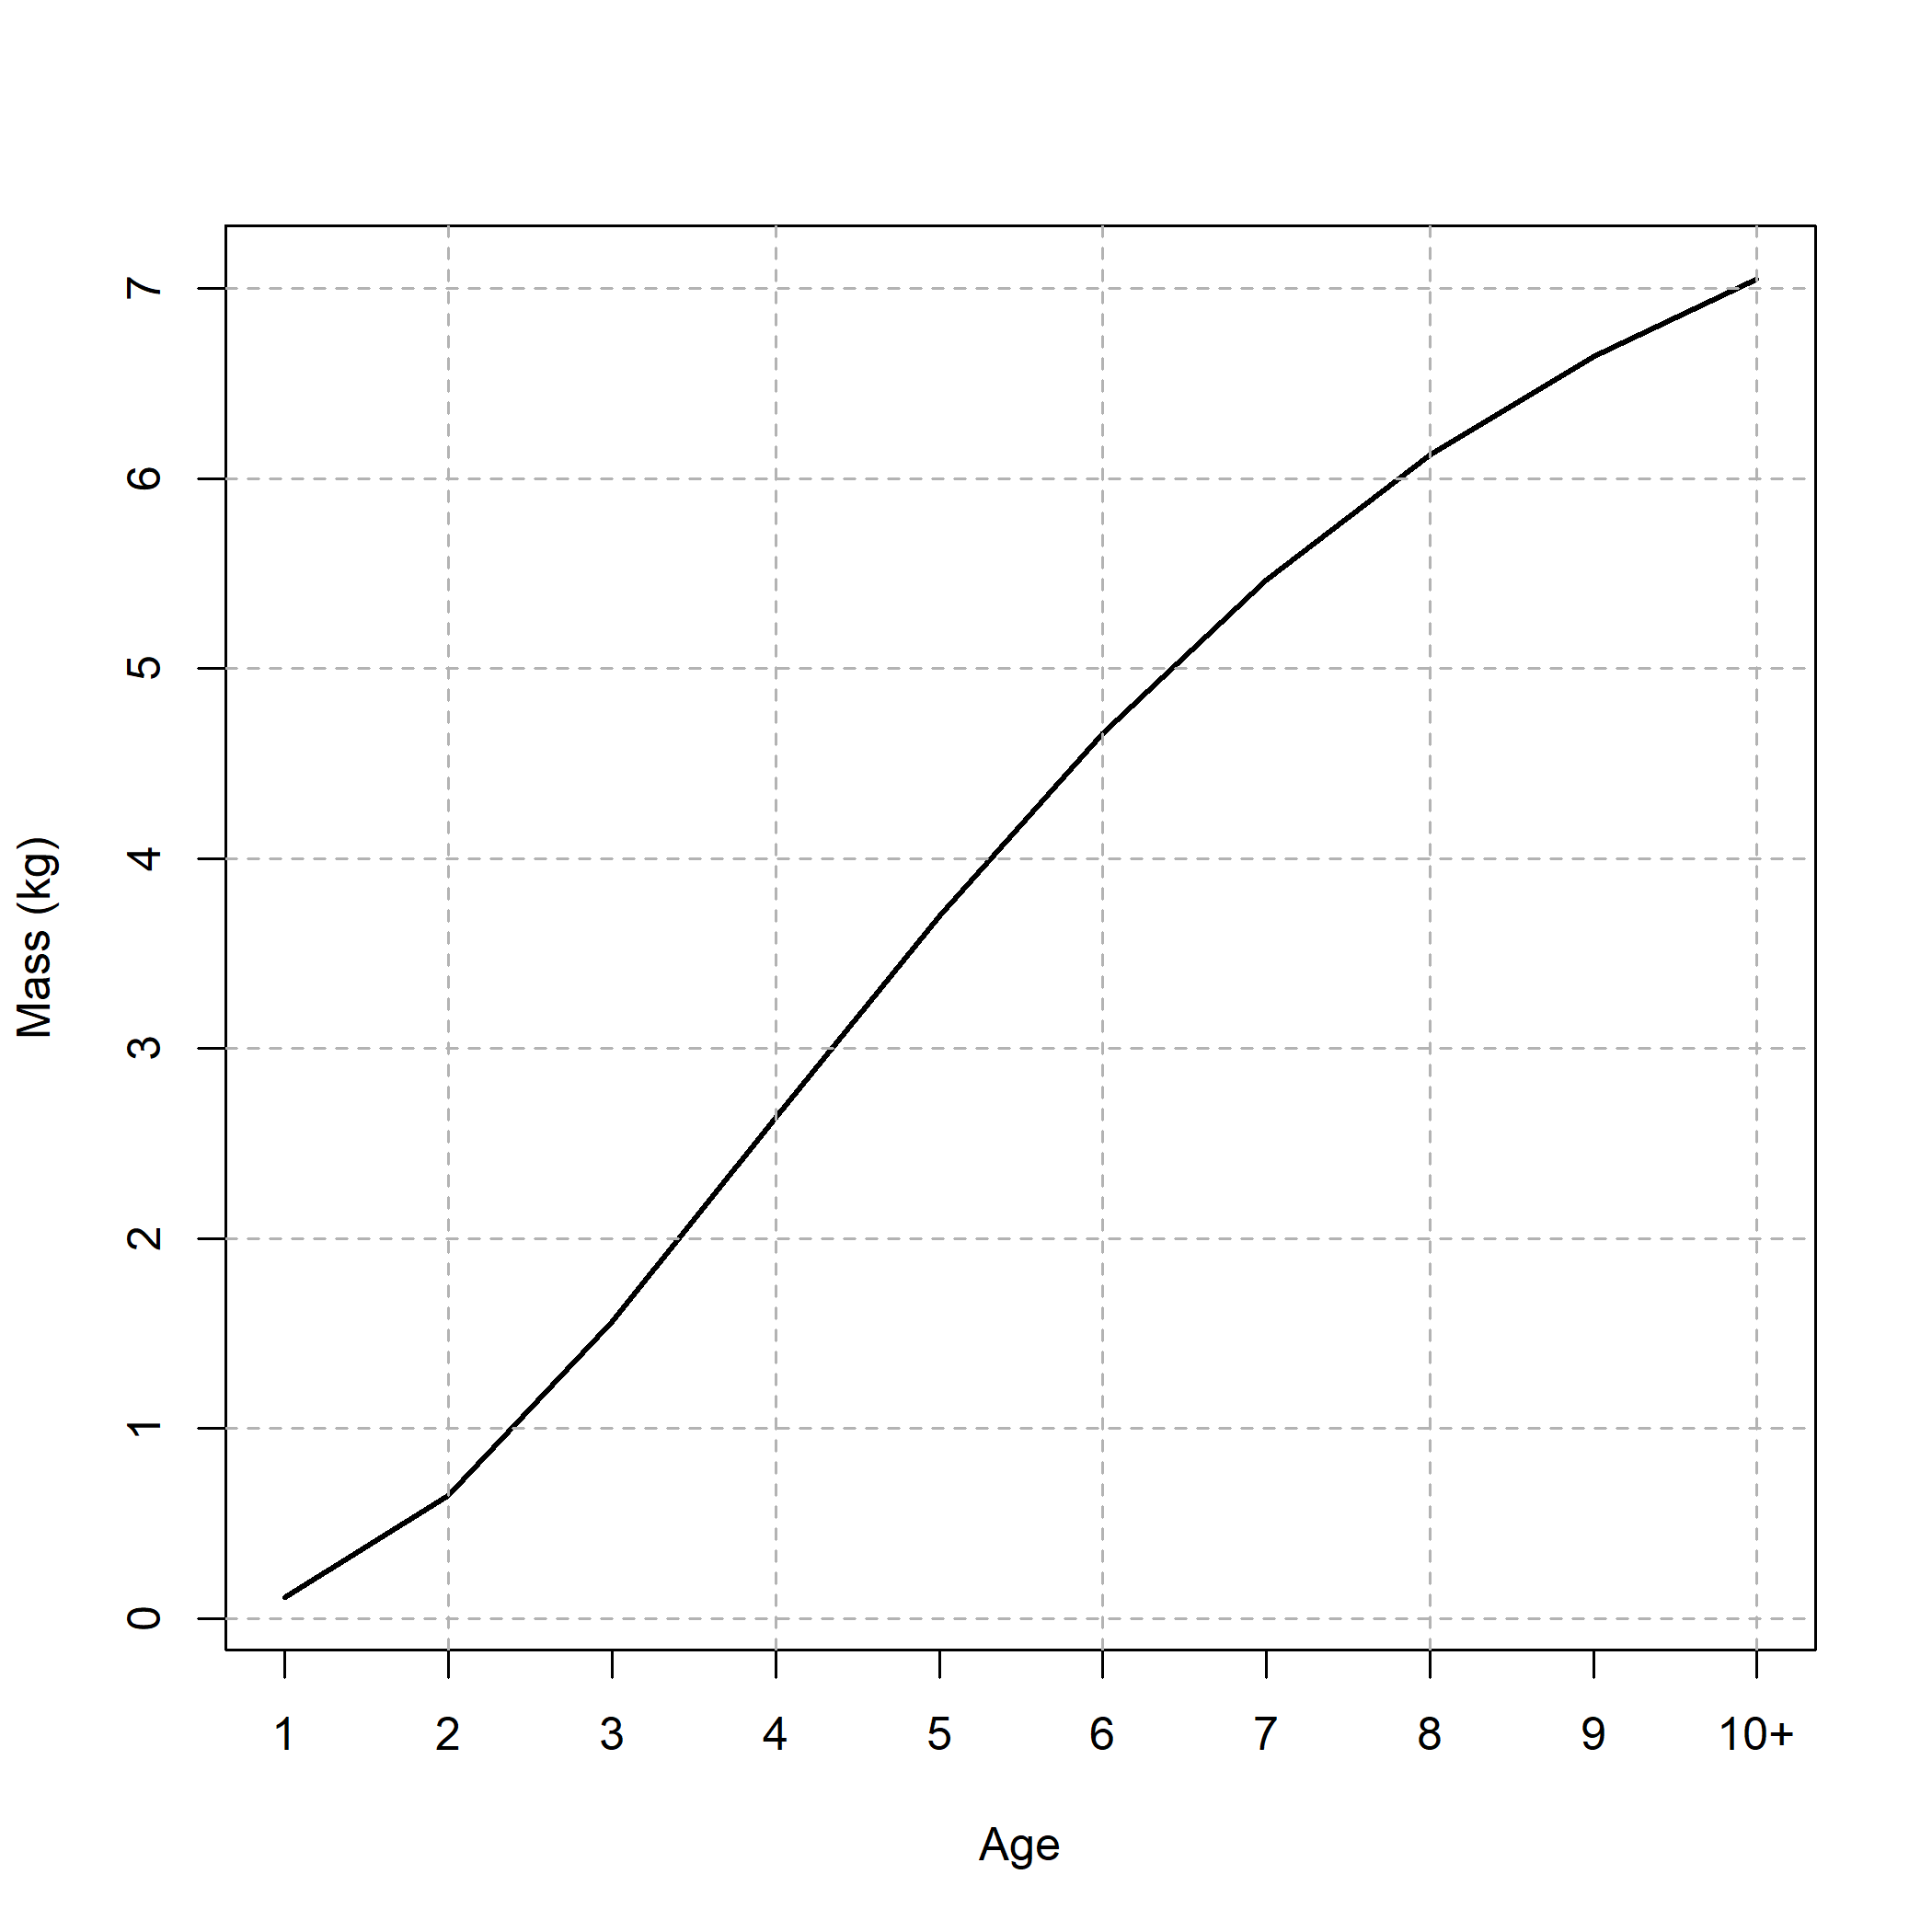
\includegraphics[width = \textwidth]{om_waa.png}
\end{center}
\end{figure}

We assumed a Beverton-Holt stock recruit function with constant
pre-recruit mortality parameters for all operating models. All
post-recruit productivity components are constant in the NAA and survey
catchability process error operating models. Therefore steepness and
unfished recruitment are also constant over the time period for those
operating models \citep{millerbrooks21}. We specified unfished
recruitment = \(R_0 = e^{10}\) and \(\Fmsy = \Fspr[40] = 0.348\) equated
to a steepness of 0.69 and \(\alpha=0.60\) and
\(\beta = 2.4 \times 10^{-5}\) for the \[
N_{1,y} = \frac{\alpha \text{SSB}_{y-1}}{1 + \beta \text{SSB}_{y-1}} 
\] Beverton-Holt parameterization (Figure \ref{om_sr}). For OMs without
process errors on natural mortality we assumed the rate was assumed 0.2.
For OMs with process errors on natural mortality the mean rate was 0.2.

\begin{figure}
\caption{The Beverton-Holt stock recruit relationship assume for all operating models.}\label{om_sr}
\begin{center}
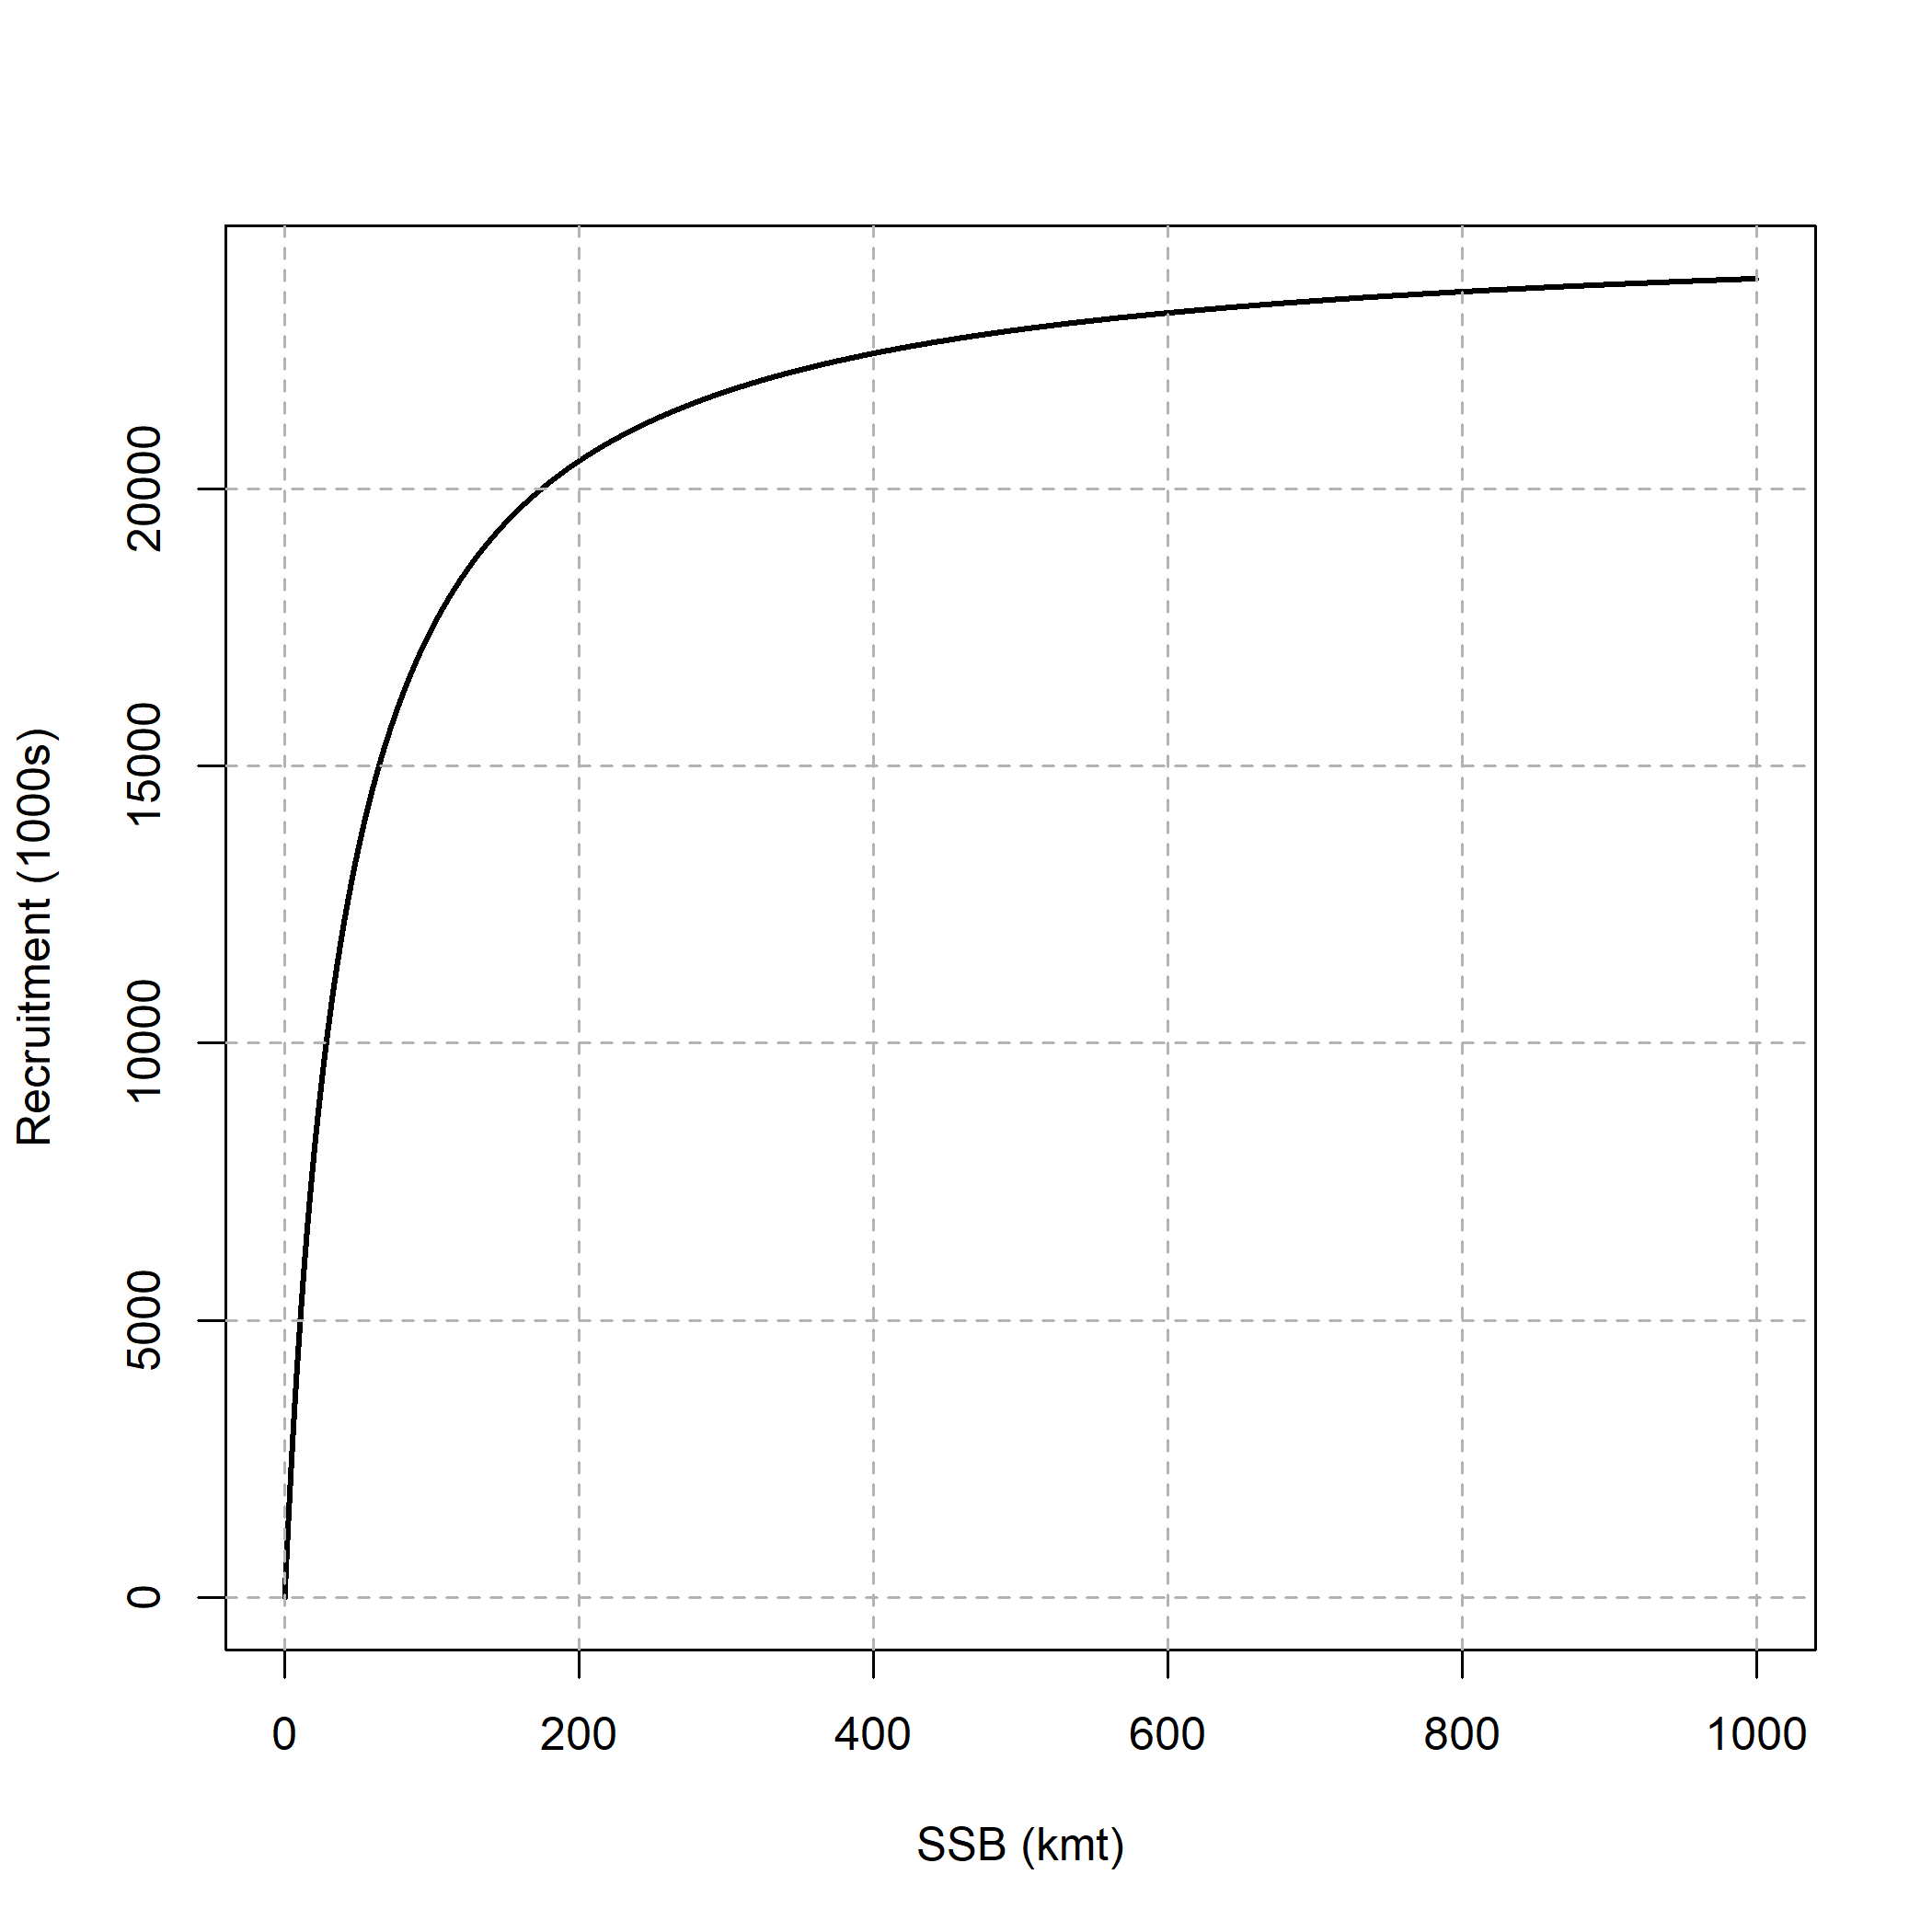
\includegraphics[width = \textwidth]{om_sr.png}
\end{center}
\end{figure}

Two alternative fishing histories were used for operating models. In the
first scenario, the stock experiences overfishing for the first 20 years
and fishing at \Fmsy for the last 20 years. In the second scenario, the
stock is fished at \Fmsy for the entire time period. The magnitude of
the overfishing assumptions is based on average estimates of overfishing
for NE groundfish stocks from \citet{wiedenmannetal19}.
\Citet{legaultetal23} also used similar approaches to defining fishing
mortality histories for operating models.

Initial population was configured at the equilibrium distribution
fishing at either \(F = 2.5\times \Fmsy\) or \(F = \Fmsy\) for the two
alternative fishing histories. That is for a deterministic model, the
age composition would not change over time when the fishing mortality
was constant at the respective level.

For operating models with time-varying random effects or covariate
effects on M, steepness is not constant, but we used the same alpha and
beta parameters as other operating models this equates to a steepness
and R0 at the mean of the time series process for M. For operating
models with time-varying random effects for fishery selectivity,
\Fmsy is also not constant however we use the same F history as other
operating models which corresponds to Fmsy at the mean selectivity
parameters.

\hypertarget{environmental-covariate}{%
\subsubsection*{Environmental covariate}\label{environmental-covariate}}
\addcontentsline{toc}{subsubsection}{Environmental covariate}

In the WHAM model, environmental covariates are assumed to be described
as state-space processes with annual observations of the true latent
covariate. The latent covariate is assumed to be Gaussian AR1 \[
E_y|E_{y-1} \sim \text{N}\left(\mu_\text{Ecov}\left(1-\rho_\text{Ecov}\right) + \rho_\text{Ecov} E_{y-1}, \sigma^2_\text{Ecov}\right)
\] with marginal mean \(\mu_\text{Ecov}\) and variance
\(\frac{\sigma^2_\text{Ecov}}{1-\rho_\text{Ecov}^2}\). The configuration
of the latent environmental covariate in the operating models have one
of two alternate assumptions about the marginal standard deviation and
autocorrelation parameter:

\begin{itemize}
\item marginal standard deviation $\in \{0.1, 0.5\}$
\item AR1 correlation $\rho_\text{Ecov} \in \{0, 0.9\}$
\end{itemize}

The observations of the latent environmental covariate are assumed to be
unbiased and Gaussian \[
\text{ecov}_y|E_y \sim \text{N}\left(E_y,\sigma^2_\text{ecov}\right)
\] The standard deviation of the environmental observations in the
operating models is one of two values:

\begin{itemize}
\item standard deviation $\in \{0.1, 0.5\}$
\end{itemize}

Figure \ref{om_ecov_example} provides example simulations of the latent
process and observations under the alternative configurations.

\begin{figure}
\caption{Example simulations of environmental covariate latent processes and observations with different levels of observation error, and different assumptions about variability of the latent process.}\label{om_ecov_example}
\begin{center}
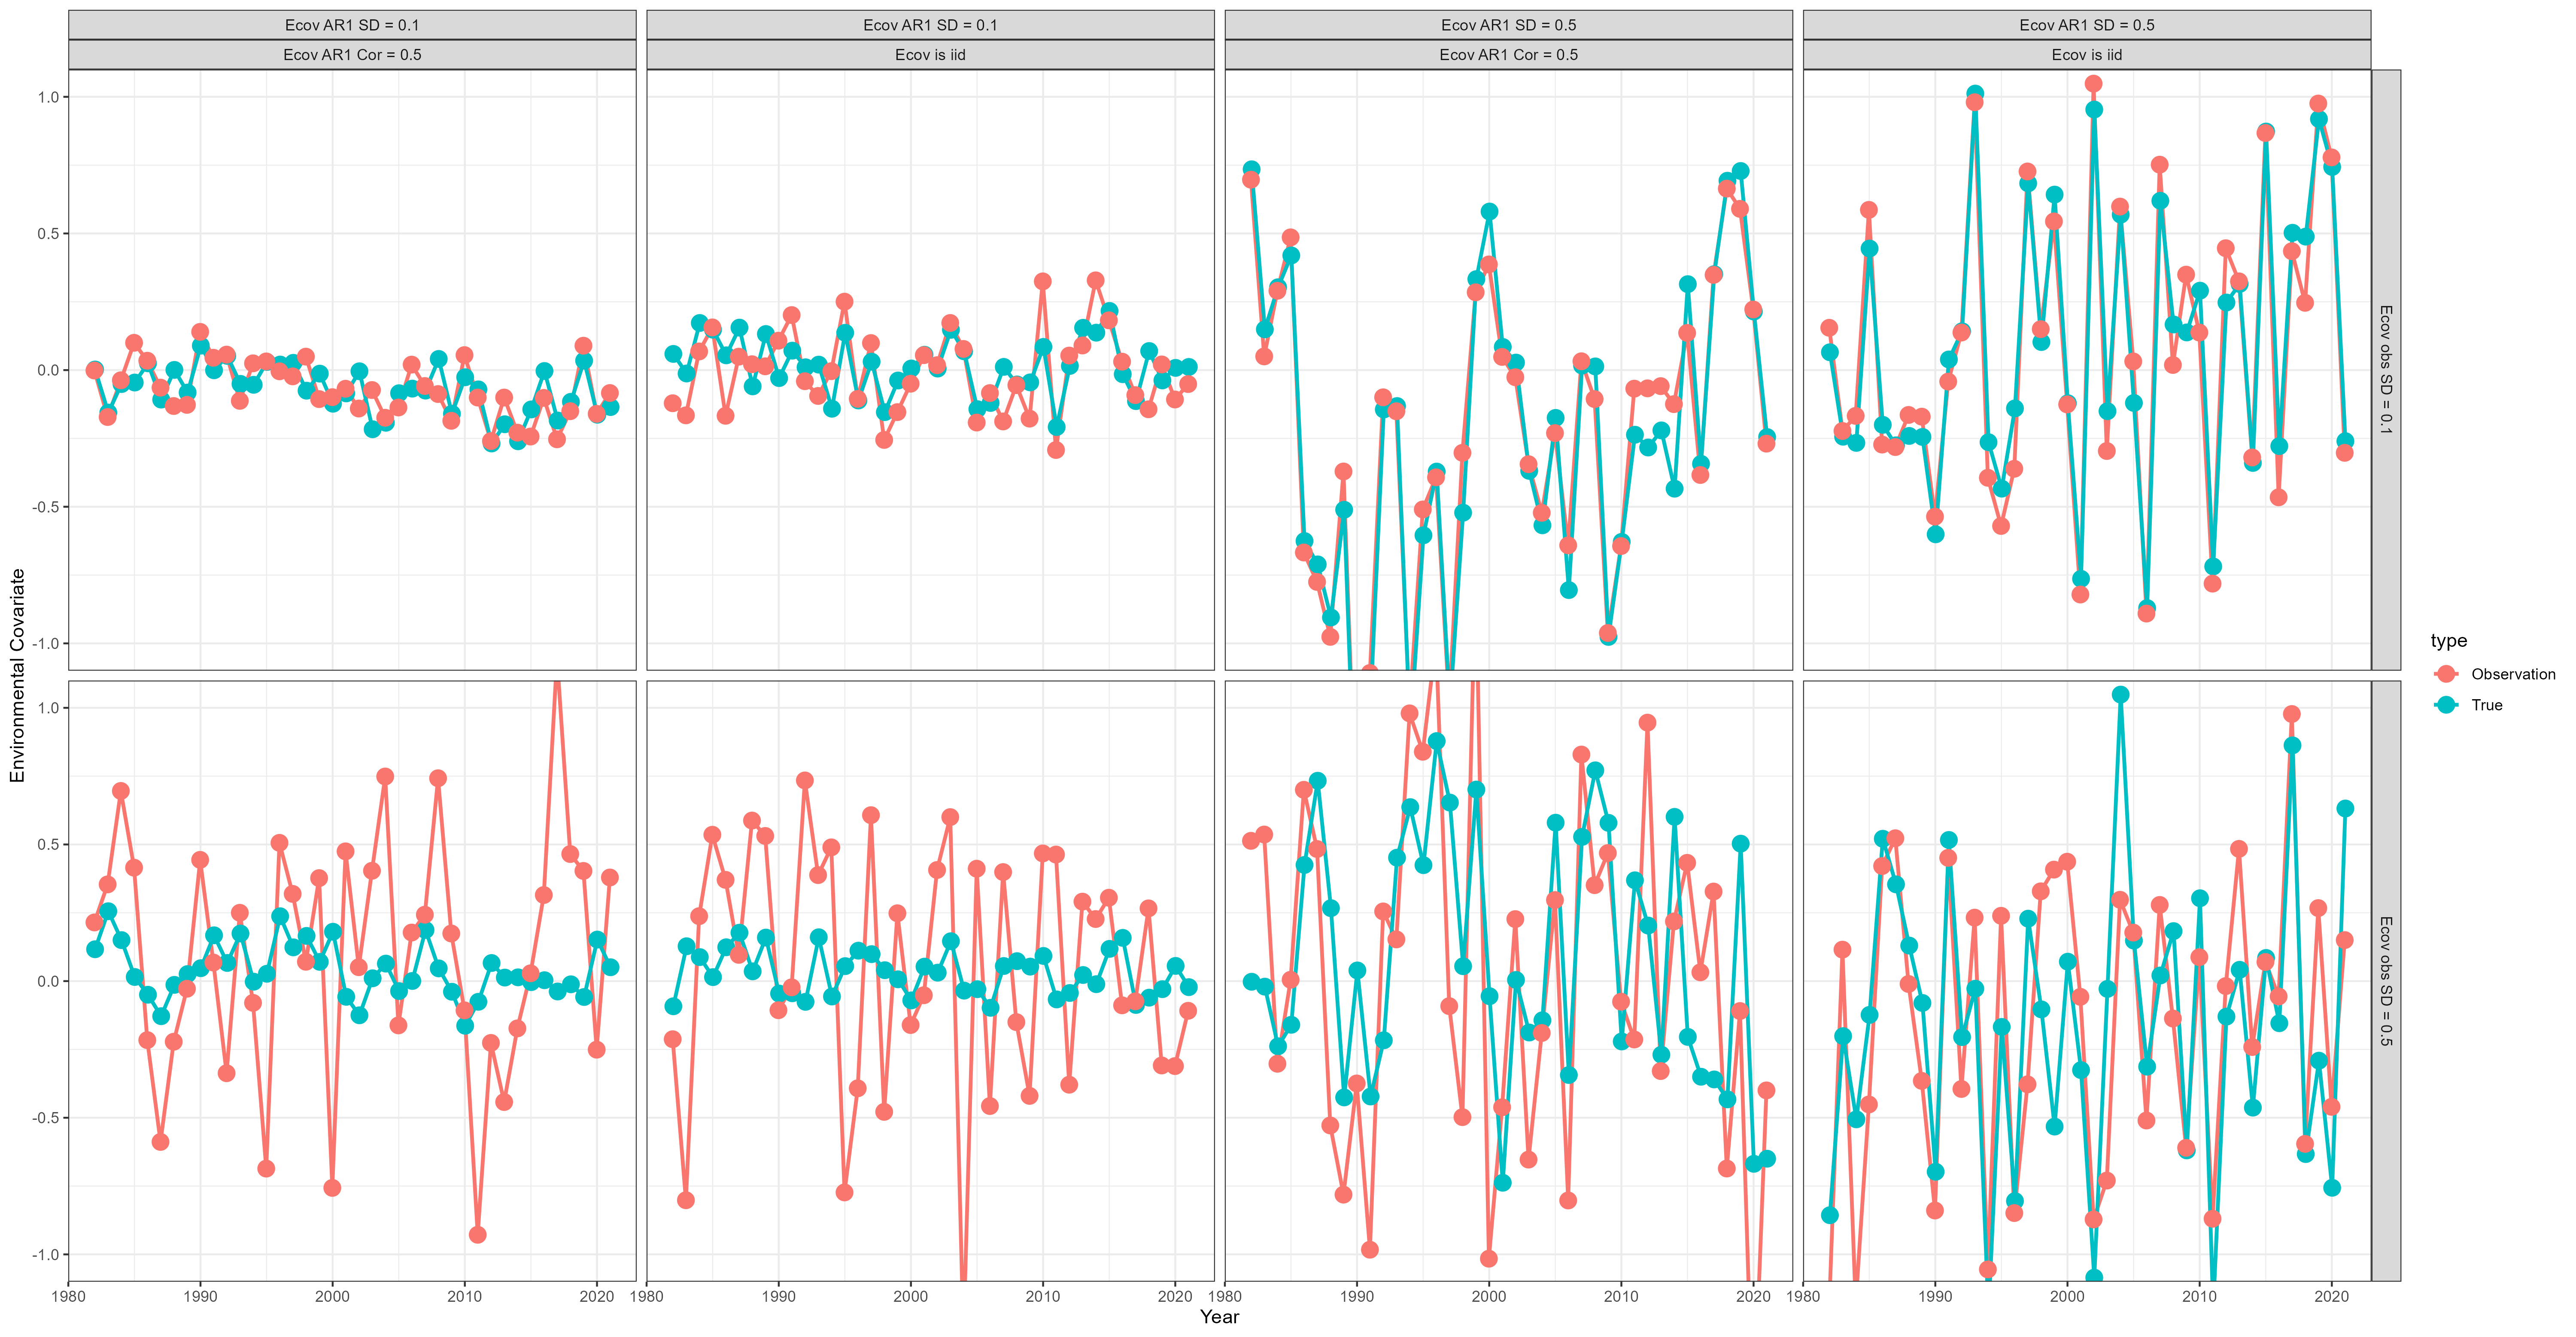
\includegraphics[width = \textwidth]{Ecov_true_obs_example.png}
\end{center}
\end{figure}

\hypertarget{random-effects-on-recruitment-survival-and-natural-mortality}{%
\subsubsection*{Random effects on recruitment, survival, and natural
mortality}\label{random-effects-on-recruitment-survival-and-natural-mortality}}
\addcontentsline{toc}{subsubsection}{Random effects on recruitment,
survival, and natural mortality}

Internally, WHAM treats natural mortality as a log-transformed parameter
\[
\log M_y = \beta_M + \beta_{\text{Ecov}} E_y + \epsilon_{M,y}
\] that is a linear combination of a mean \(\beta_M\) and any annual
covariate \(\beta_{\text{Ecov}}\) and random effects marginally
distributed as
\(\epsilon_{M,y} \sim \text{N}\left(0,\sigma_M^2\right)\).

The covariate effect is one of 3 alternative values in the operating
models:

\begin{itemize}
\item $\beta_\text{Ecov} \in \{0,0.25,0.5\}$
\end{itemize}

The alternative configurations of random effects on recruitment, natural
mortality, survival

\begin{itemize}
\item uncorrelated random effects on R and survival with $\sigma_R = 0.5$, marginal standard deviation of survival of older age clases of 0.3
\item uncorrelated random effects on R and survival with $\sigma_R = 0.5$, marginal standard deviation of natural mortality of 0.3
\end{itemize}

\hypertarget{fleets}{%
\subsubsection*{Fleets}\label{fleets}}
\addcontentsline{toc}{subsubsection}{Fleets}

We assumed a single fleet operating year round for catch observations
with logistic selectivity for the fleet with \(a_{50} = 5\) and slope =
1 (Figure \ref{om_mean_selectivity}). This selectivity is was used to
define \Fmsy for the Beverton-Holt stock recruitment parameters above.
We assumed a logistic-normal distribution for the age-composition
observations for the fleet.

\begin{figure}
\caption{The selectivity at age assumed for the fishing fleet in operating models without selectivity random effects. The mean selectivity at age across time for the fishing fleet in operating models with selectivity random effects.}\label{om_mean_selectivity}
\begin{center}
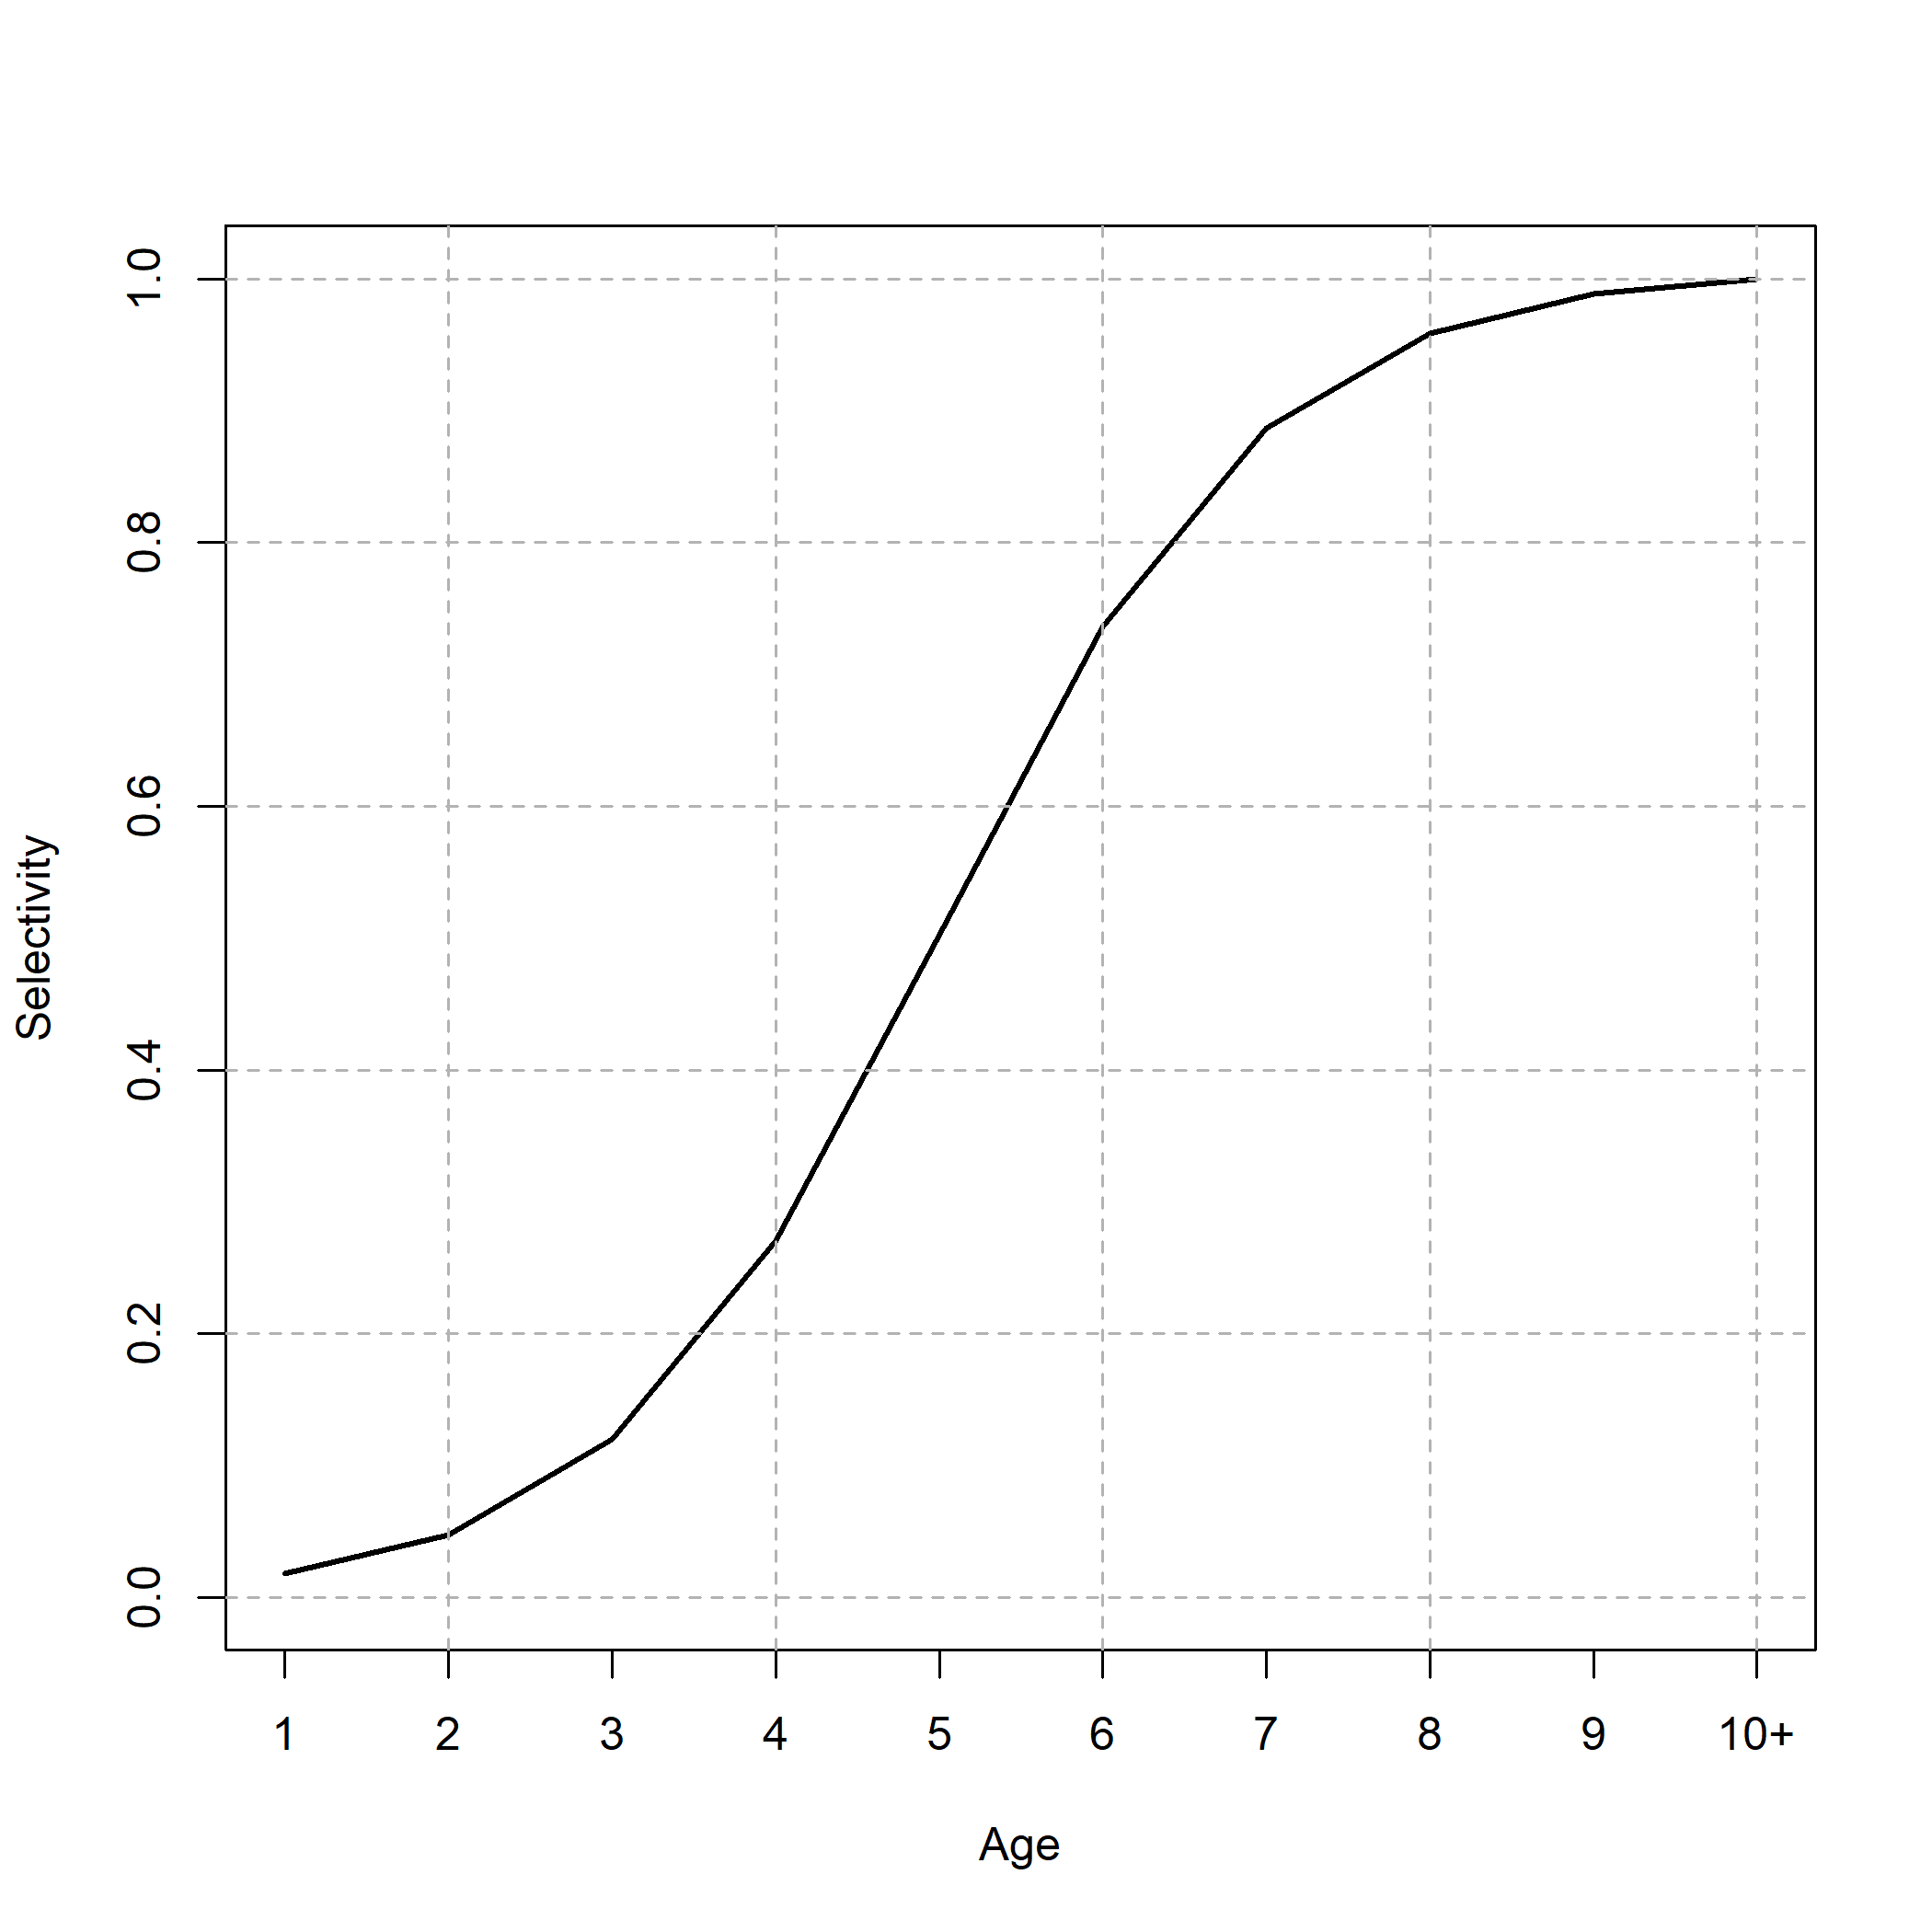
\includegraphics[width = \textwidth]{om_mean_selectivity.png}
\end{center}
\end{figure}

\hypertarget{indices}{%
\subsubsection*{Indices}\label{indices}}
\addcontentsline{toc}{subsubsection}{Indices}

Two time series of surveys are assumed and observed in numbers rather
than biomass for the entire 40 year period with one occurring in the
spring (0.25 way through the year) and one in the fall (0.75 way through
the year). Actually we have it currently configured that both occur 0.5
way through the year. Catchability of both surveys are assumed to be
0.1. Like the fishing fleet, we assumed logistic selectivity for both
indices with \(a_{50} = 5\) and slope = 1 and a logistic-normal
distribution for the age-composition observations.

\hypertarget{observation-uncertainty}{%
\subsubsection*{Observation Uncertainty}\label{observation-uncertainty}}
\addcontentsline{toc}{subsubsection}{Observation Uncertainty}

Standard deviation for log-aggregate catch was 0.1. There were two
levels of observation error variance for indices and age composition for
both indices and fleet catch. A low uncertainty specification assumed
standard deviation of both series of log-aggregate index observations
was 0.1 and the standard deviation of the logistic-normal for age
composition observations was 0.3 In the high uncertainty specification
the standard deviation for log-aggregate indices was 0.4 and that for
the age composition observations was 1.5. For all estimating models,
standard deviation for log-aggregate observations was assumed known
whereas that for the logistic-normal age composition observations was
estimated.

The factorial combinations of fishing histories, index and age
composition observation error assumptions, latent environmental
covariate and observation assumptions, covariate effects on natural
mortality, and sources of process error (R, R+S, R+M) results in 288
different operating models.

\hypertarget{estimating-models}{%
\subsection*{Estimating models}\label{estimating-models}}
\addcontentsline{toc}{subsection}{Estimating models}

For each data set simulated from an operating model 12 estimating models
were fit. There were three factors defining the configuration of each
estimating model

\begin{itemize}
\item whether the mean natural mortality $\beta_M$ was estimated or assumed known ($\log 0.2$)
\item whether an environmental effect $\beta_\text{Ecov}$ was estimated or not (fixed at 0)
\item whether the process errors were just on recruitment (R), on recruitment and survival (R+S) or on recruitment and natural mortality (R+M)
\end{itemize}

The configuration of the process errors in the estimating models matched
the corresponding options in the operating models. For example, if R+S
was assumed for both the estimating and operating model, the assumptions
about process errors matched. The environmental covariate observations
were included in all estimation models to ensure comparability of
information criteria. The observation error variance of the
environmental observations and aggregate catch and indices were all
assumed known at the true values.

Simulations were all carried out on the University of Massachusetts
Green High-Performance Computing Cluster. Code for completing the
simulations and summarization of results can be found at
github.com/timjmiller/SSRTWG/ecov\_study/mortality. We used the wham
package version 1.X.X (commit 77bbd94).

\hypertarget{measures-of-reliability}{%
\subsection*{Measures of reliability}\label{measures-of-reliability}}
\addcontentsline{toc}{subsection}{Measures of reliability}

The first measure of reliability we investigated was frequency of
convergence when fitting each estimating model to the simulated data
sets. There are various ways to assess convergence of the fit. We
summarized 5 alternative categories of convergence. 1. Did the
optimization routine (stats::nlminb) complete without error? 2. Did the
stats::nlminb convergence flag = 0 indicate successful convergence? 3.
Was the maximum absolute value of the gradient of the log-likelihood
\textless{} \(1\times10^{-6}\)? 4. Did TMB::sdreport provide non-NA
values for all fixed effects standard errors? 5. Did TMB::sdreport
provide all standard errors \textless{} 100?

The first convergence criterion assesses whether the model crashes. The
third is a measure that assesses how flat the likelihood is at the
optimized point of the likelihood surface. The fourth and fifth criteria
are specific to the hessian-based standard error reporting provided by
TMB. the TMB::sdreport function will sometimes return standard error
estimates even when the calculated hessian is not invertible (fourth
criterion). It will also provide large standard errors for some
parameters that are not estimated well or are near bounds on the
transformed scale that is of primary interest. For example, variance
parameters for random effects can often be estimated near 0 when the fit
suggests no variation in the random effects or, equivalently, that the
model without random effects is better.

\hypertarget{aic-for-model-selection}{%
\subsubsection*{AIC for model selection}\label{aic-for-model-selection}}
\addcontentsline{toc}{subsubsection}{AIC for model selection}

We measured the frequency of correct model selection using marginal AIC.
For a given operating model we the set of models that were considered
all made the same assumptions on whether or not to estimate M and
whether a stock-recruit function is assumed.

\hypertarget{bias}{%
\subsubsection*{Bias}\label{bias}}
\addcontentsline{toc}{subsubsection}{Bias}

We calculated relative errors of various quantities for each fitted
estimation model for the \(i\)th simulated data set as \[
{\text{RE}_i}\left(\theta\right) = \frac{\widehat \theta_i - \theta_i}{\theta_i}
\] and measured bias as the median relative error and constructed 95\%
confidence intervals using the binomial distribution approach as in
\citet{stockmiller21}.

\hypertarget{results}{%
\section*{Results}\label{results}}
\addcontentsline{toc}{section}{Results}

\hypertarget{convergence-performance}{%
\subsection*{Convergence performance}\label{convergence-performance}}
\addcontentsline{toc}{subsection}{Convergence performance}

\begin{landscape}
\begin{figure}
\caption{Probability of convergence of estimating models with alternative process error assumptions fit to simulated populations and data sets from operating models. The convergence criterion is an invertible hessian providing standard error estimates for all fixed effects parameters. Vertical lines represent 95\% confidence intervals. All estimating models estimate environmental covariate effects on natural mortality but assume the mean mortality parameter $\beta_\text{M} = \log 0.2$.}\label{convergence_M_fixed}
\begin{center}
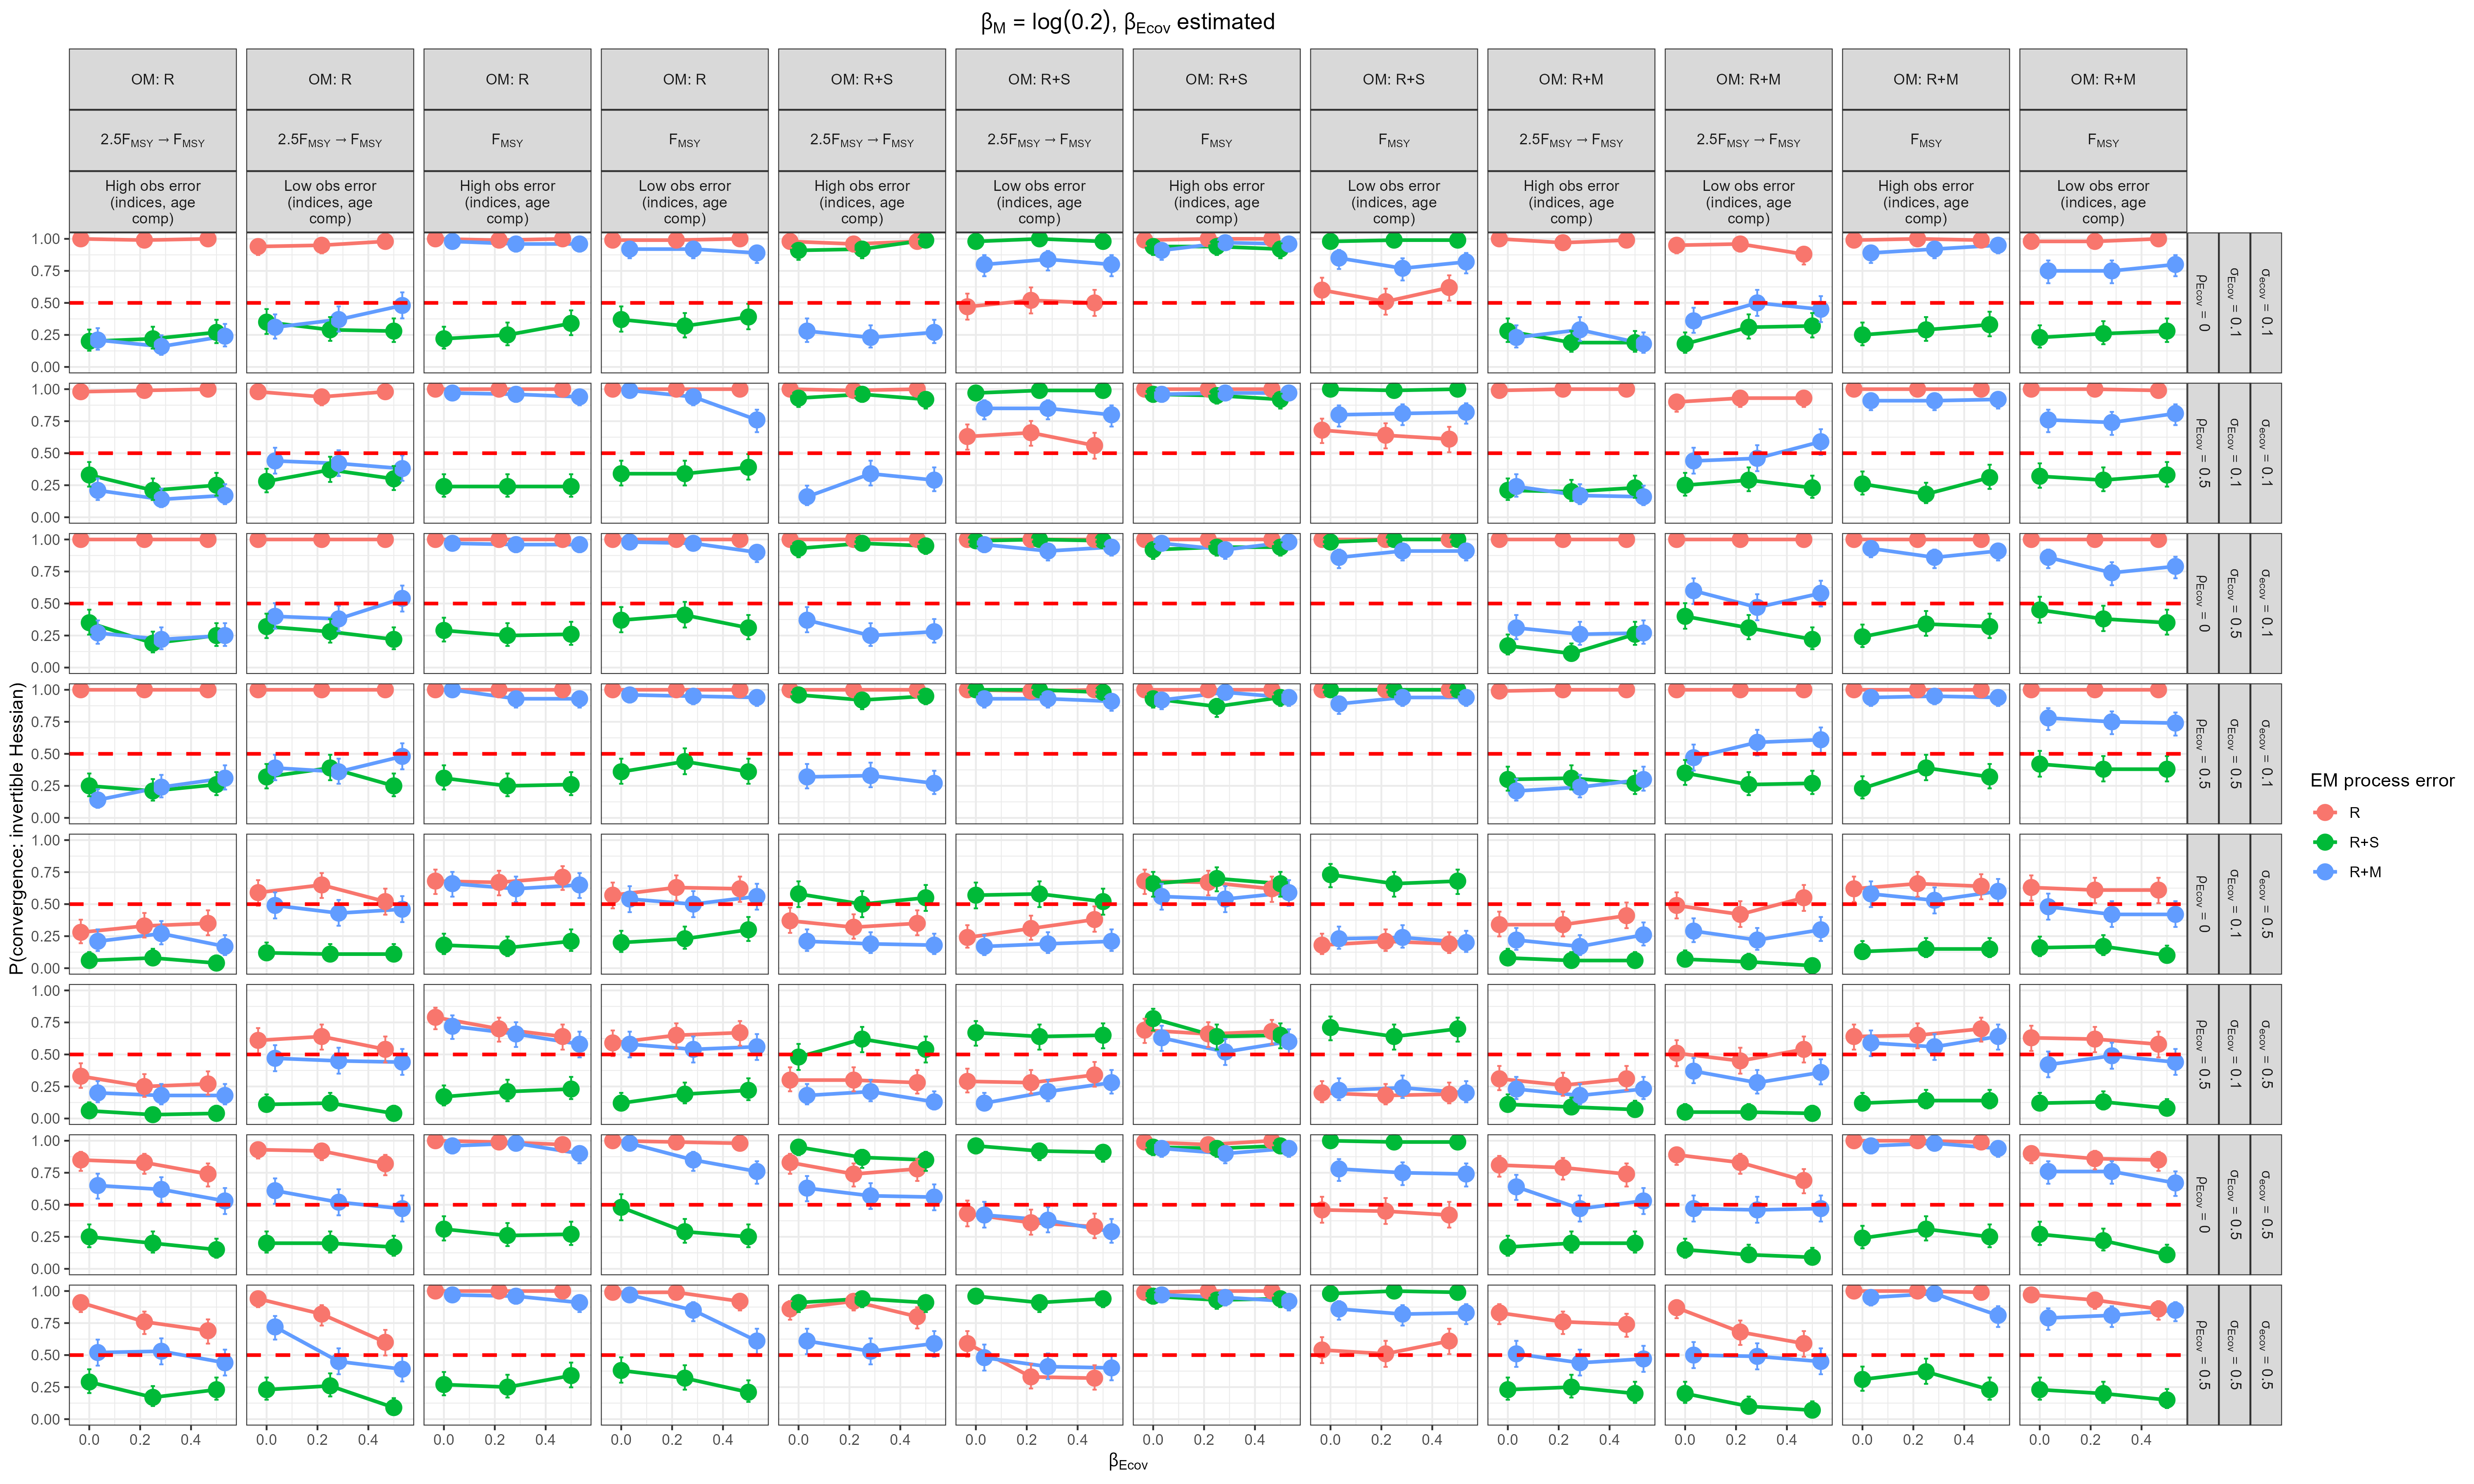
\includegraphics[width = \textwidth]{proportion_good_hessian_ecov_effect_est_M_fixed.png}
\end{center}
\end{figure}
\end{landscape}

\begin{landscape}
\begin{figure}
\caption{Probability of convergence of estimating models with alternative process error assumptions fit to simulated populations and data sets from operating models. The convergence criterion is an invertible hessian providing standard error estimates for all fixed effects parameters. Vertical lines represent 95\% confidence intervals. All estimating models estimate environmental covariate effects on natural mortality and the mean mortality parameter $\beta_\text{M}$.}\label{convergence_M_estimated}
\begin{center}
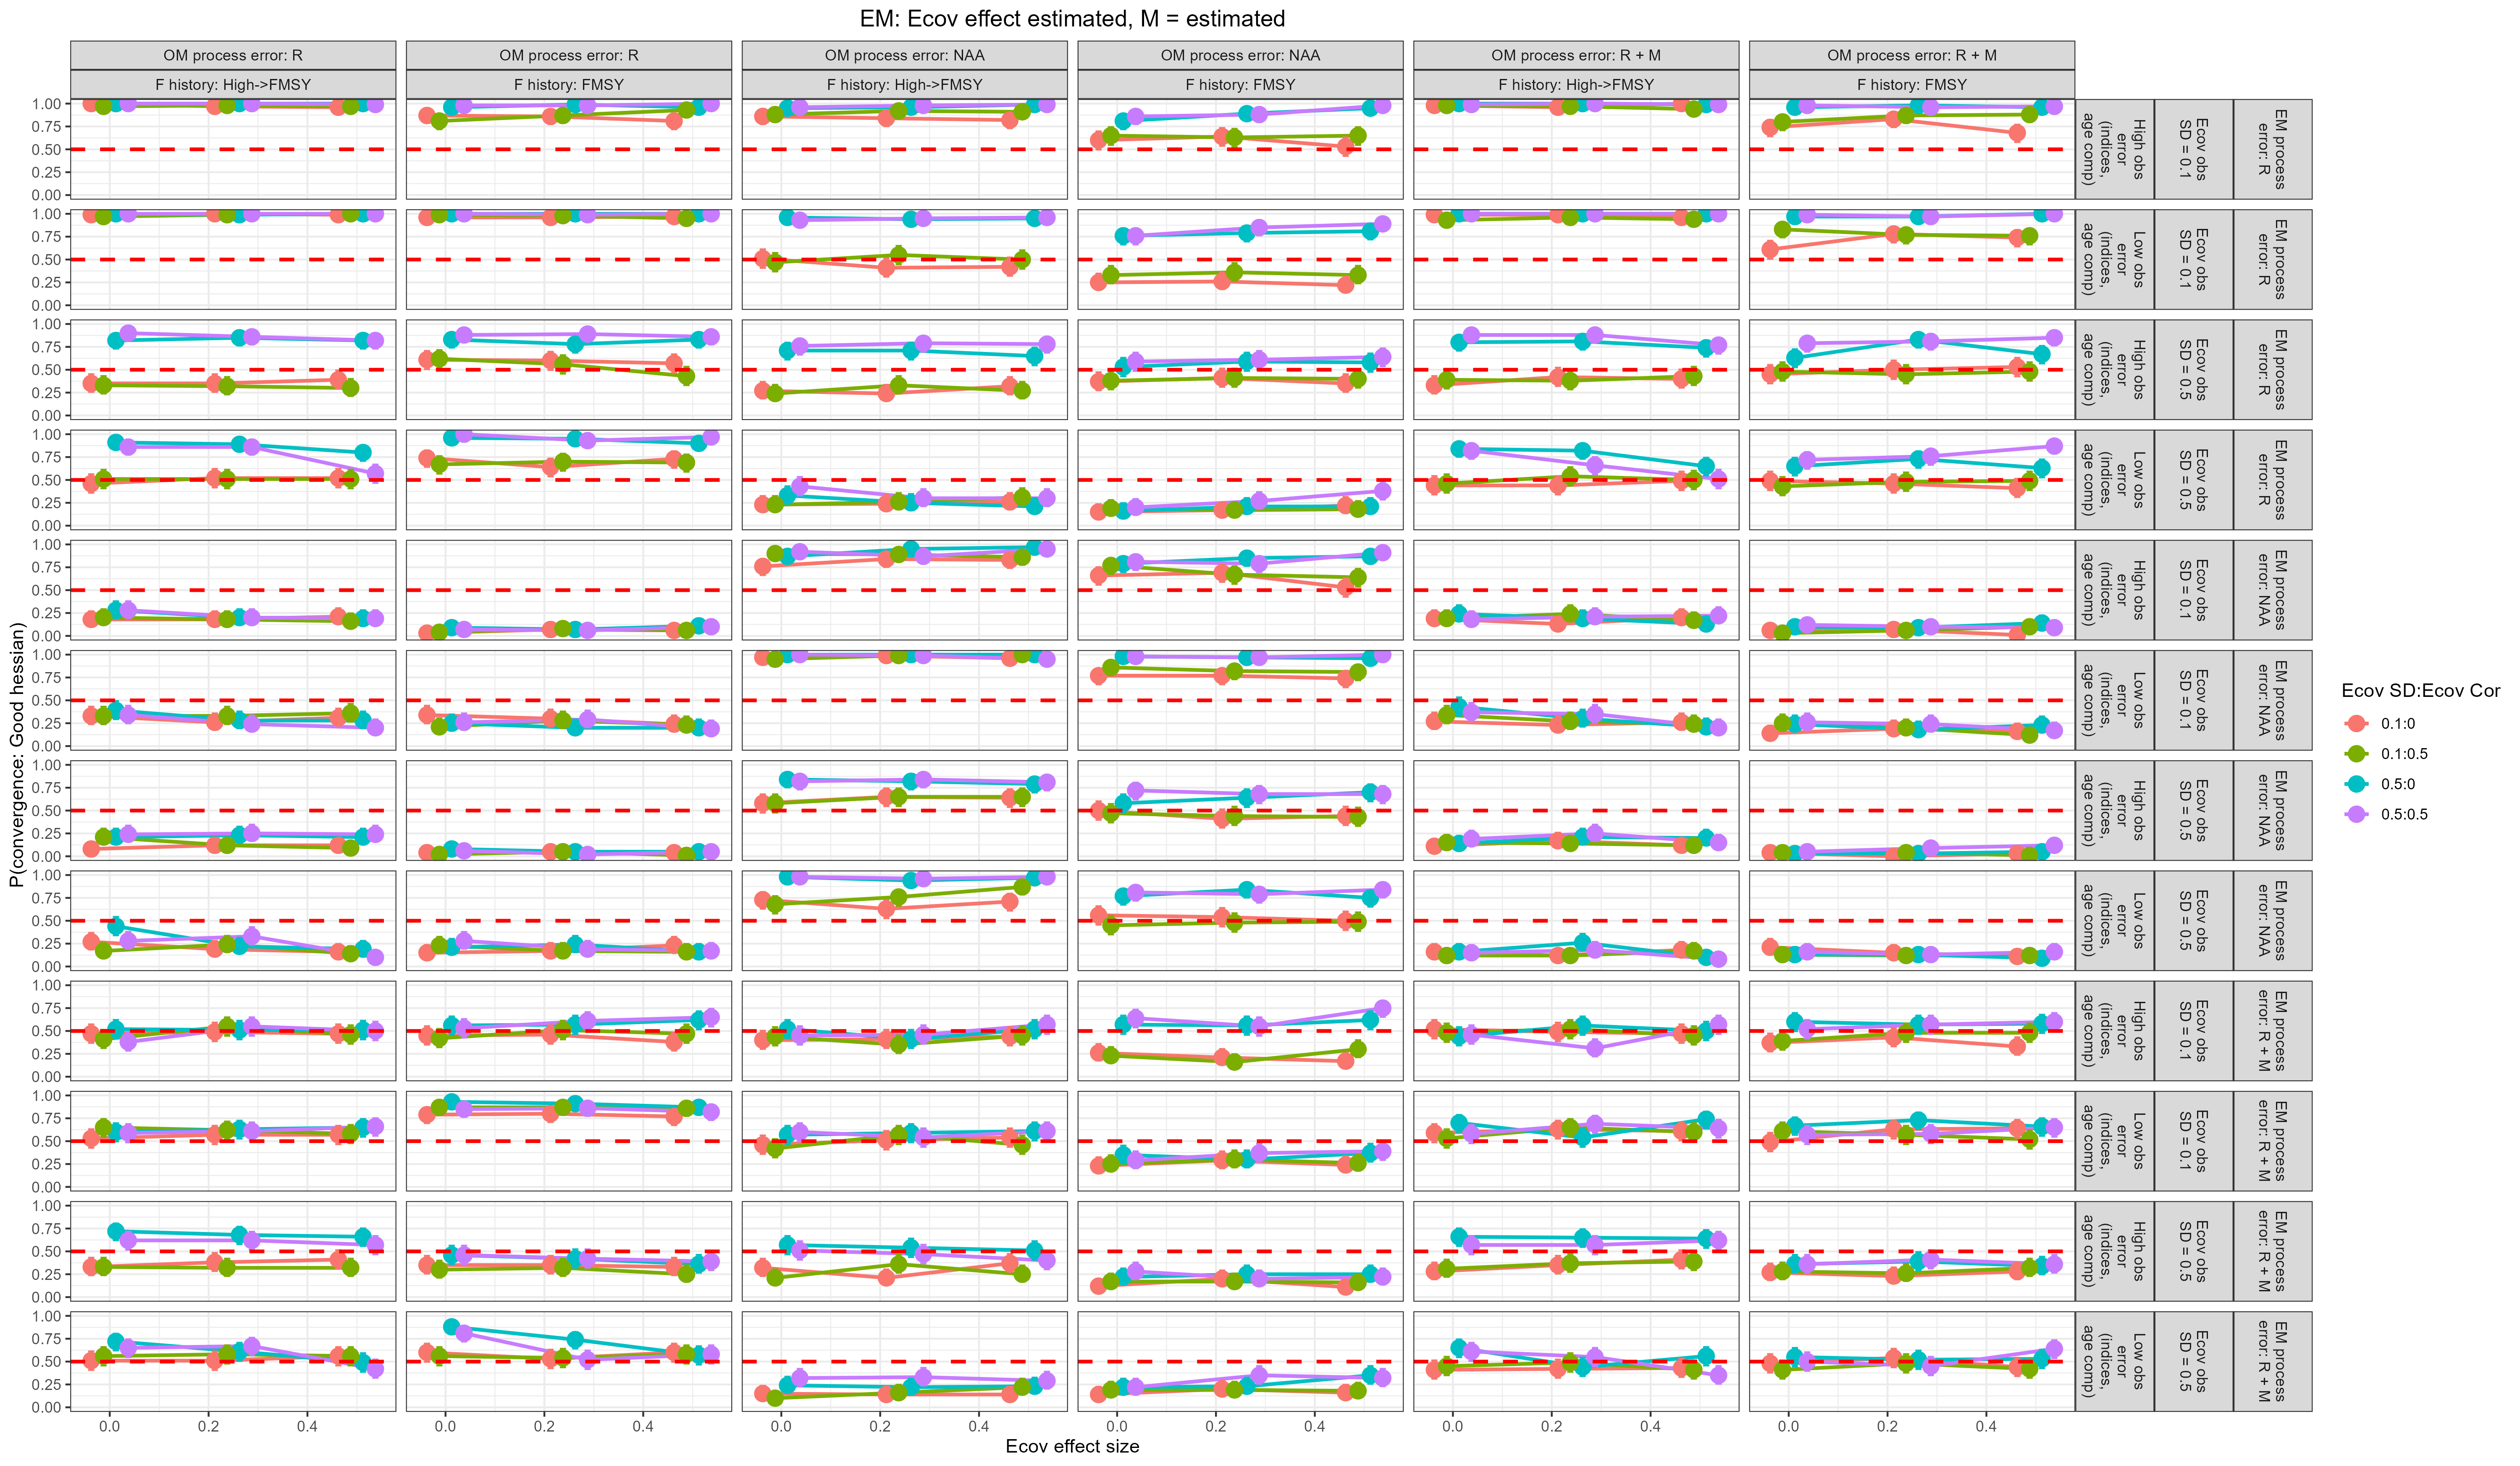
\includegraphics[width = \textwidth]{proportion_good_hessian_ecov_effect_est_M_est.png}
\end{center}
\end{figure}
\end{landscape}

\hypertarget{aic-performance}{%
\subsection*{AIC performance}\label{aic-performance}}
\addcontentsline{toc}{subsection}{AIC performance}

\begin{landscape}
\begin{figure}
\caption{Proportion of simulated data sets for each operating model where the estimation model with the lowest AIC had correct assumptions of process errors (R,R+S,R+M) and/or about whether the environmental covariate affected natural mortality. All estimating models assumed the mean mortality parameter $\beta_\text{M} = \log 0.2$.}\label{aic_rank_M_fixed}
\begin{center}
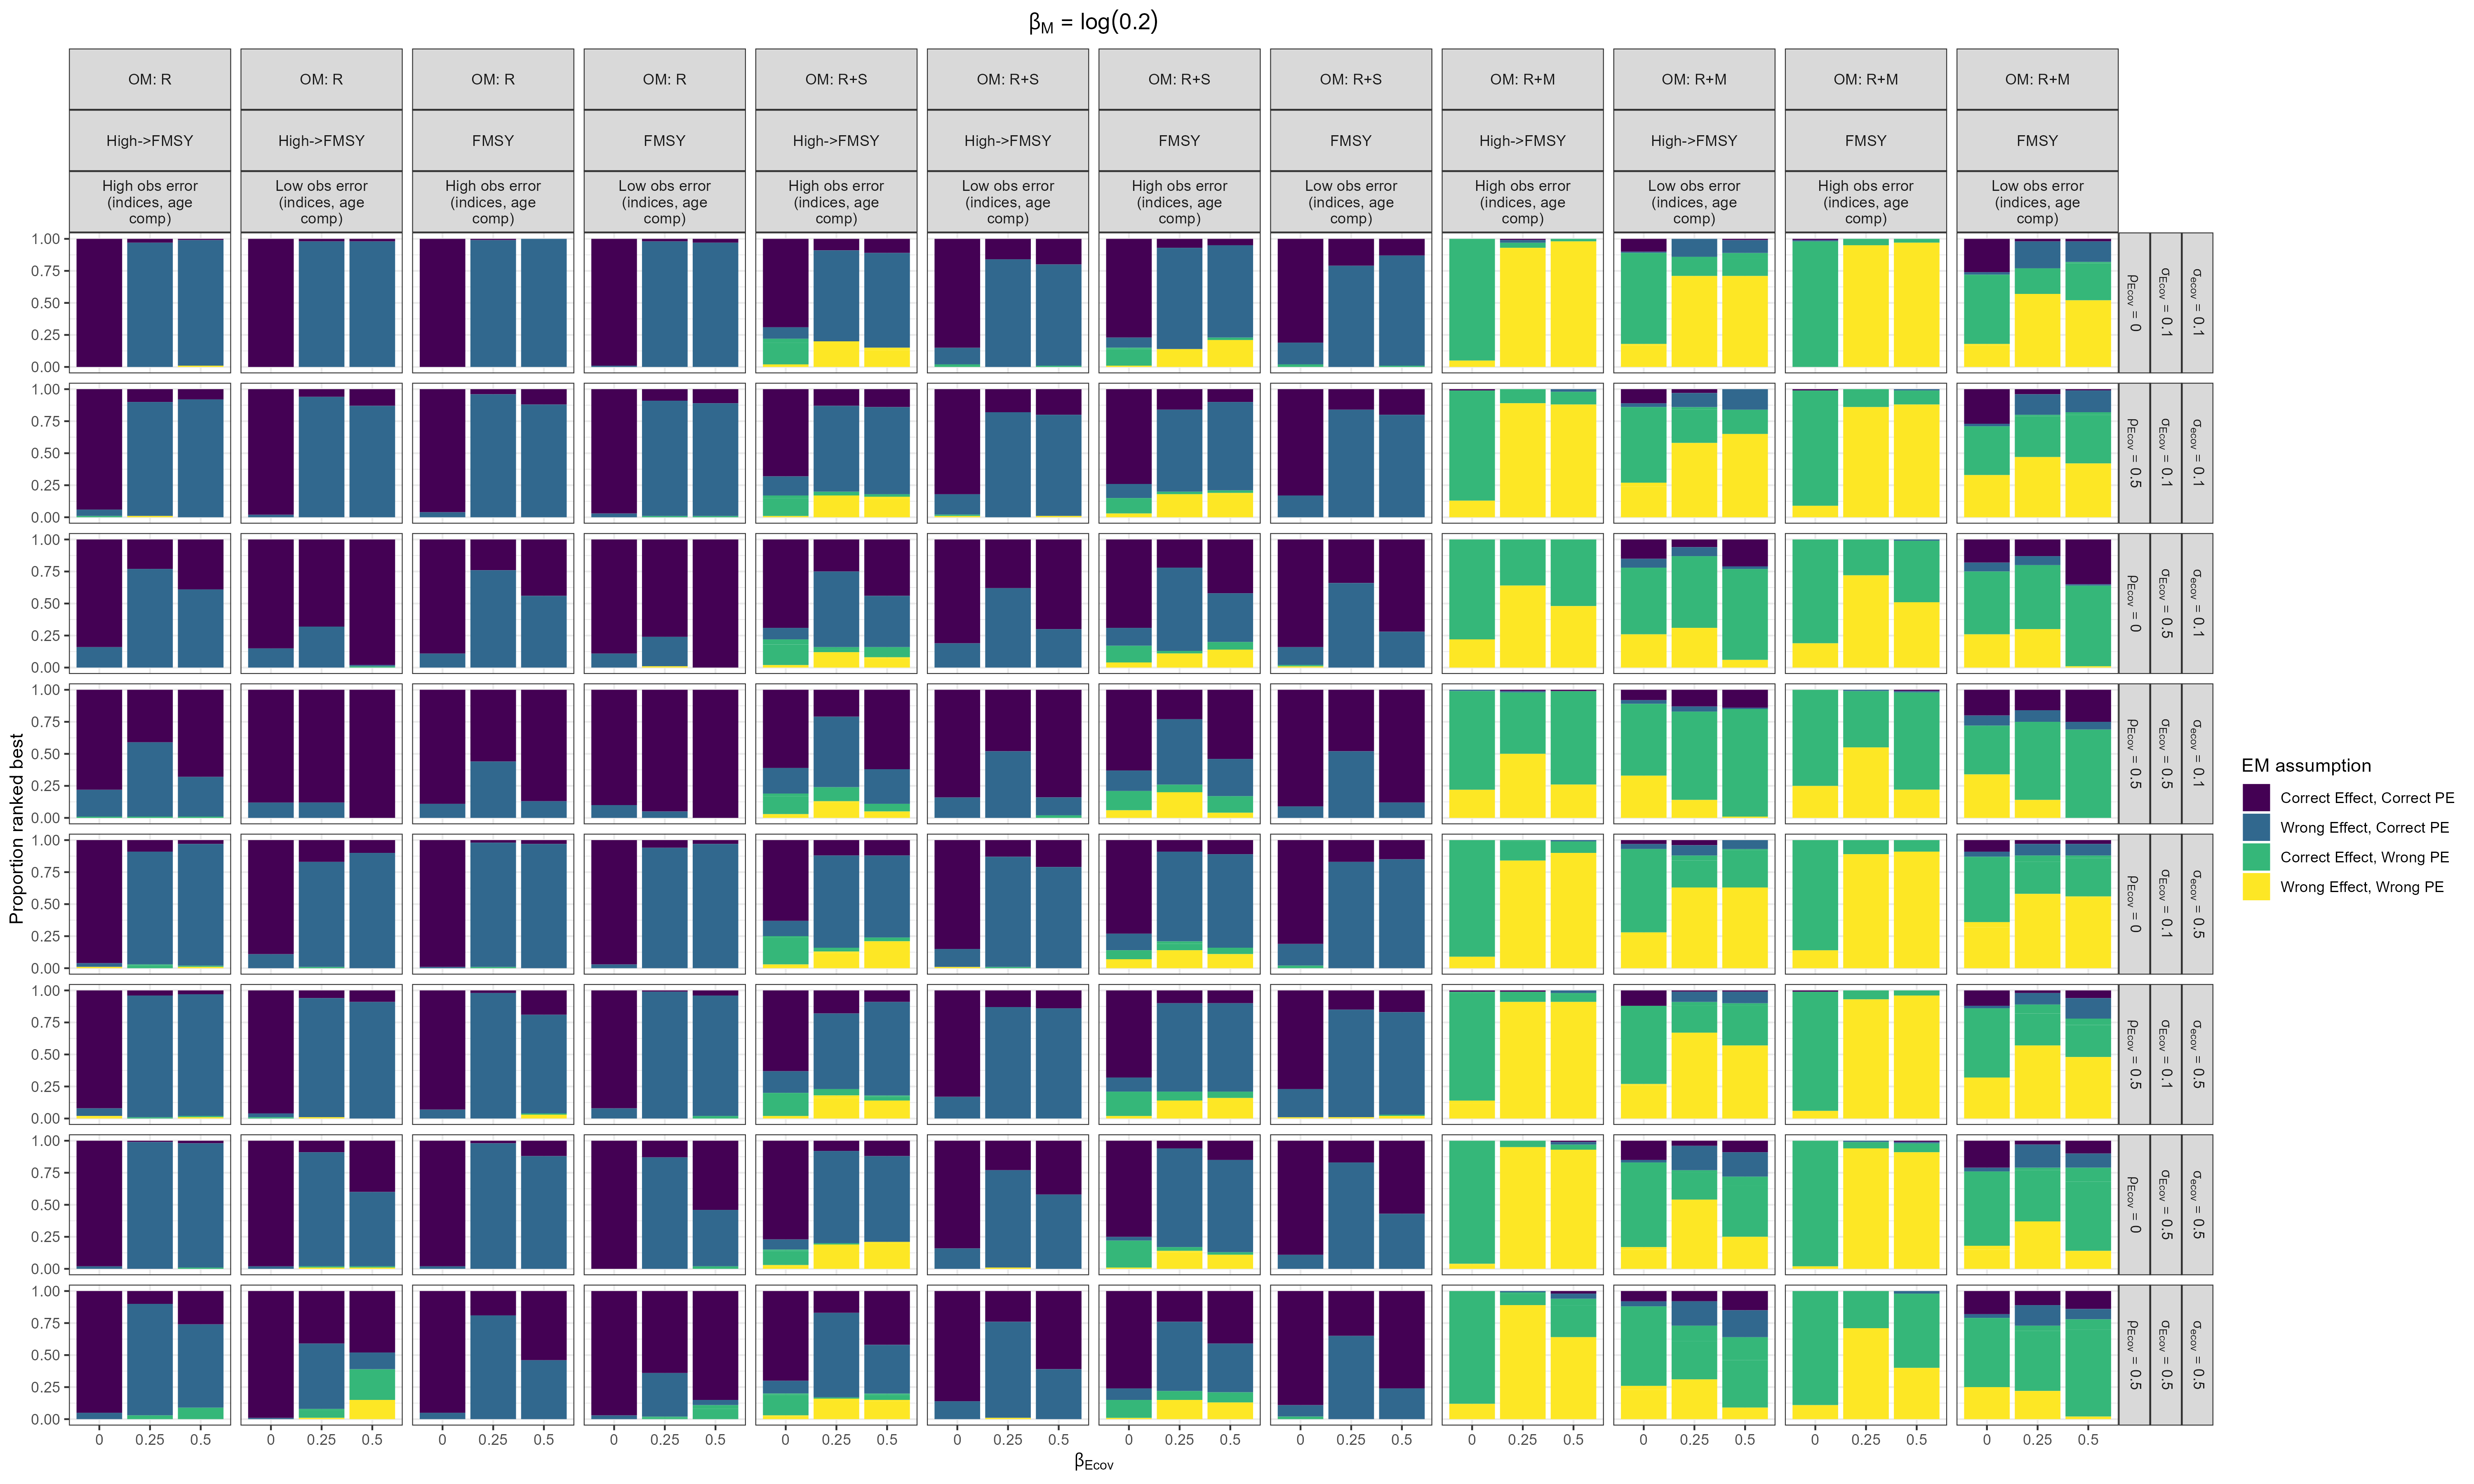
\includegraphics[width = \textwidth]{proportion_correct_PE_effect_M_fixed.png}
\end{center}
\end{figure}
\end{landscape}

\begin{landscape}
\begin{figure}
\caption{Proportion of simulated data sets for each operating model where the estimation model with the lowest AIC had correct assumptions of process errors (R,R+S,R+M) and/or about whether the environmental covariate affected natural mortality. All estimating models estimate the mean mortality parameter $\beta_\text{M}$.}\label{aic_rank_M_estimated}
\begin{center}
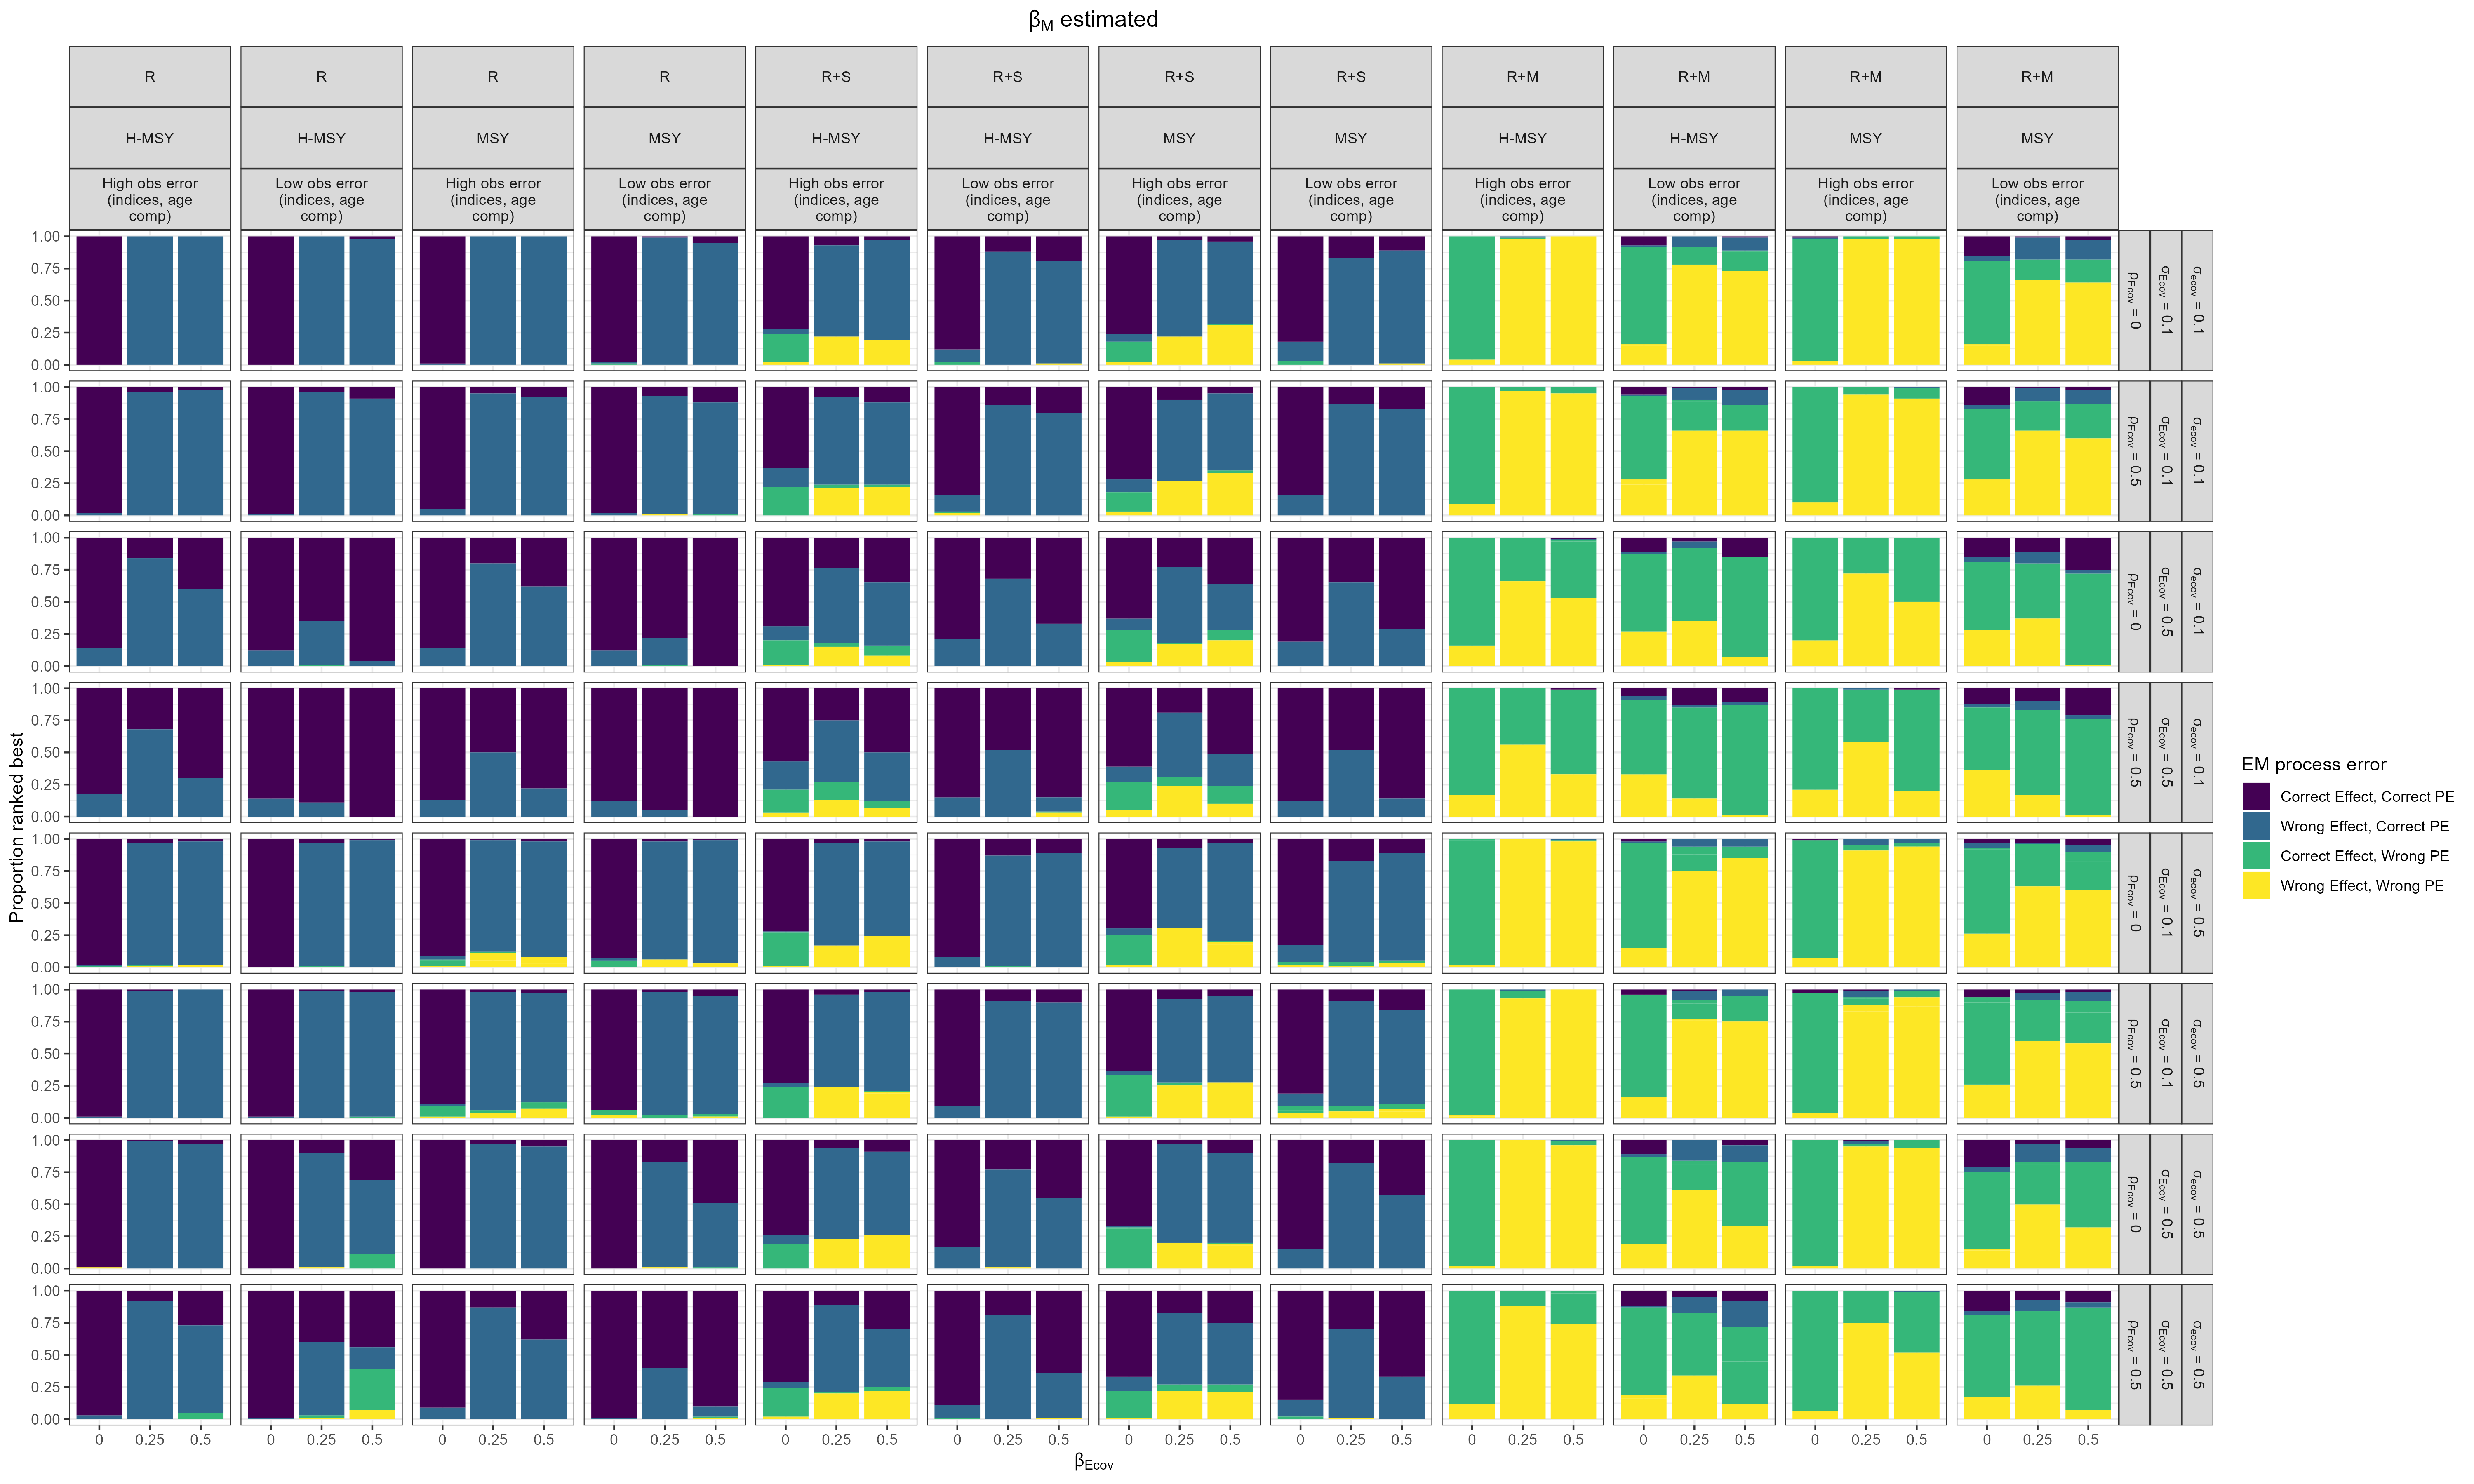
\includegraphics[width = \textwidth]{proportion_correct_PE_effect_M_estimated.png}
\end{center}
\end{figure}
\end{landscape}

\hypertarget{bias-1}{%
\subsection*{Bias}\label{bias-1}}
\addcontentsline{toc}{subsection}{Bias}

\hypertarget{discussion}{%
\section*{Discussion}\label{discussion}}
\addcontentsline{toc}{section}{Discussion}

The estimating models assumed variances of aggregate catch and index
observations was known. This approximation may be appropriate for
indices where we have a reliable estimate of uncertainty based on the
survey design (), but there may be better approaches for the aggregate
catch such as an informed prior on the standard errors with realistic
bounds.

\hypertarget{acknowledgements}{%
\section*{Acknowledgements}\label{acknowledgements}}
\addcontentsline{toc}{section}{Acknowledgements}

This work was funded by NOAA Fisheries Northeast Fisheries Science
Center.

\pagebreak

\bibliography{paper}

\hypertarget{refs}{}
\begin{CSLReferences}{0}{0}
\end{CSLReferences}

\pagebreak

\end{document}
